\chapter{Data parsing as bars}
\label{chapterDataParsing}
The previous chapters used low frequency data. In particular, daily data was 
used which just means that after every trading day a single observation is 
gathered. On the other side of the spectrum rests high frequency data, which 
can be viewed as the purest form of financial data.\\

However, raw data does not mean that everything will work better. To feed 
this data to ML algorithms, it must be preprocessed in a way that 
superfluous information is discarded and useful parts are kept.\\

Before diving into the actual data manipulation, a brief explanation will be 
given to understand better where the term ``data bars'' come. As López de 
Prado states in~\cite{AdvFML}, most ML algorithms assume a table 
representation of the extracted data and the tables' rows are often referred 
by practitioners as ``bars''.

\section{Data bars}
In section \ref{sec:highFrequencyData} of chapter \ref{chapterIntroFinDat}, 
it was seen that raw financial data comes in ticks, and thus, inhomogenous 
in time. In order to structure data, samples of the price will be recorded 
whenever a certain event happens (time elapsed, price change, etc.). In 
consequence, different events will give rise to different type of bars.\\

A useful concept that will help understand how data bars arose is the 
concept of stochastic clock, proposed by Clark 
in~\cite{clark1973subordinated}. This clock will only ``show the time'' when 
certain events happen. For instance, a volume clock will only show the time 
when $M_{\text{volume}}$ units are exchanged. Hence, volume bars will be 
recorded whenever the volume clock ``shows the time''.\\

In the following subsections, the bars that Marcos López de Prado designated 
as standard in \cite{AdvFML} will be presented. 

\subsection*{Time bars}
These bars consist of sampling the price every $M_{\text{time}}$ minutes 
(e.g. every 1, 5, 30 minutes or longer). Note that daily data lays in this 
category since it records the price of an asset once a day.\\

One of the drawbacks of time bars is the fact that they ignore periods of 
high activity. That is, if one was sampling every 30 minutes and the bulk of 
trading occurred during the first and last 15 minutes of the trading 
session, then information would be lost.

\subsection*{Tick Bars}
As the name implies, the sampling will occur every certain amount of ticks 
($M_{\text{ticks}}$). Since ticks are directly related with transactions, 
during periods of high activity more samples will be gathered.\\

The problem with sampling data using ticks is the lack of control over the 
number of stocks traded. To put it another way, if one wanted to buy 5 
stocks and there were 5 separate offers of size 1 that matched, then the 
whole operation would count as 5 transactions. However, if there was an offer 
of size 5 that matched, it would be recorded as 1 transaction, even though 
the same number of stocks have been exchanged.\\

That is why López de Prado states in~\cite{AdvFML} that order fragmentation 
introduces arbitrariness in the number of ticks.

\subsection*{Volume bars}
Volume bars will sample the price every time $M_{\text{volume}}$ stocks are 
exchanged. This will certainly help with the issue outlined with tick bars. 
In this type of bars the amount of transactions will not matter since it 
only cares about the actual amount of securities traded.\\

Also, note that one of the great virtues of volume bars is the fact that 
they will sample the price correctly in moments of high activity. In 
particular, whenever a lot of stocks are traded, plenty of bars will be 
recorded, while in a low activity environment few bars will be gathered.

\subsection*{Dollar bars}
Before introducing these bars one should know what dollar volume is: 
$d_t := v_t \cdot p_t$. At first glance, one could infer that sampling every 
time a certain dollar volume ($M_{\text{dollar}}$) is traded will lead to 
bars similar to volume ones.\\

That is true to a certain extent because if $p_t$ stays fairly constant, 
then accounting for a constant, they will sample in a similar fashion. 
However, if the stock presents high volatility, volume bars will under 
sample periods of high prices. To be specific, dollar bars can distinguish 
300 stocks being exchanged at 80\$ ($ d_t = 24,000\$ $) rather than at 70\$ 
($ d_t = 21,000\$ $).\\

\section{Data}
The security that will be used for this chapter is called \textbf{IVE}, 
which trades in the NYSE (New York Stock Exchange) Arca market. This asset 
tracks the S\&P500, which is an index that comprises the 500 most important 
US stocks.\\

Having said that, the data used will be the tick data of IVE from 2013-01-02 
to 2013-12-31. It contains 550,697 rows that include information on: price, 
bid, ask, and volume. To get an idea of the general structure of the data 
used, refer to table \ref{tab:tickData} which shows a few ticks from day 
2013-01-02.

\section{Sampling}
Having presented the tick data that will be used, the next step is 
determining the hyperparameters $M_{\text{ticks}},\ M_{\text{volume}},\ 
M_{\text{dollar}}$ and $M_{\text{time}}$, which are responsible of the 
sample gathering. Once the samples are collected the daily average of bars 
($\bar{n}^{\text{daily}}$) will be calculated. Hence, every $M$ directly 
determines $\bar{n}^{\text{daily}}$.\\

Before showing the values of $M$ used, one should bear in mind that 
processing the huge dataset and creating the bars takes a considerable 
amount of time ($\approx$ 3 hrs). Therefore, ``brute force'' is not feasible 
to choose the values of $M$. However, what has been done is the following:

\begin{itemize}
	\item Choose a sensible $M$. For example, López de Prado 
	in~\cite{volumeClock} uses $\frac{1}{50}$ of the average daily volume as
	$M_{\text{volume}}$.

	\item Shift $M$ until the fitted pdf of log-returns resembles more of a 
	normal pdf (see section \ref{sec:normalLogRet} for further details).
\end{itemize}

Having said that, the final hyperparameters chosen are shown in table
\ref{tab:samplingM}.

\newpage

\begin{table}[htbp]
\caption{Sampling hyperparameters}
\label{tab:samplingM}
\centering
\begin{tabular}{ |C{2cm}|C{2cm}|C{2cm}|C{2cm}|C{2cm}| }
	\hline
	 				& Tick & Volume & Dollar & Time\\
	\hline
	$M$ & 60 ticks & 8,000 stocks & 800,000\$ & 8 min.\\
	$\bar{n}^{\text{daily}}$ & 36.42 & 73.77 & 49.20 & 49.93\\
	\hline
\end{tabular}
\end{table}

Figure \ref{fig:dataBars} shows three trading days and the samples that were 
extracted using tick, volume, dollar and time bars. Additionally, in figure 
\ref{fig:intradayDeformed} the samples of day 2013-07-10 are presented. This 
last image is really important because it symbolizes the data bars via their 
internal clock, i.e., one unit in the x-axis represents the occurrence of a 
certain event (stocks exchanged, ticks, etc.).\\

Furthermore, since it is of the utmost importance to understand how sampling 
occurs, a few remarks on figures \ref{fig:dataBars} and 
\ref{fig:intradayDeformed} will be made:
\begin{itemize}
	\item Tick bars, although not equally spaced as time bars, seem to be 
	more distributed as time passes compared to volume and dollar bars.
	
	\item Volume and dollar samples are concentrated on periods of high 
	volatility (downswings and upswings).
	
	\item In figure \ref{fig:intradayDeformed} it can be seen that tick, 
	volume and dollar bars undersample periods where the price goes 
	sideways, while they oversample the period from 14:00 to 15:00, where 
	the bulk of activity was observed.
\end{itemize}

\begin{figure}[htbp]
	\centering
	\begin{subfigure}{.5\textwidth}
		\centering
		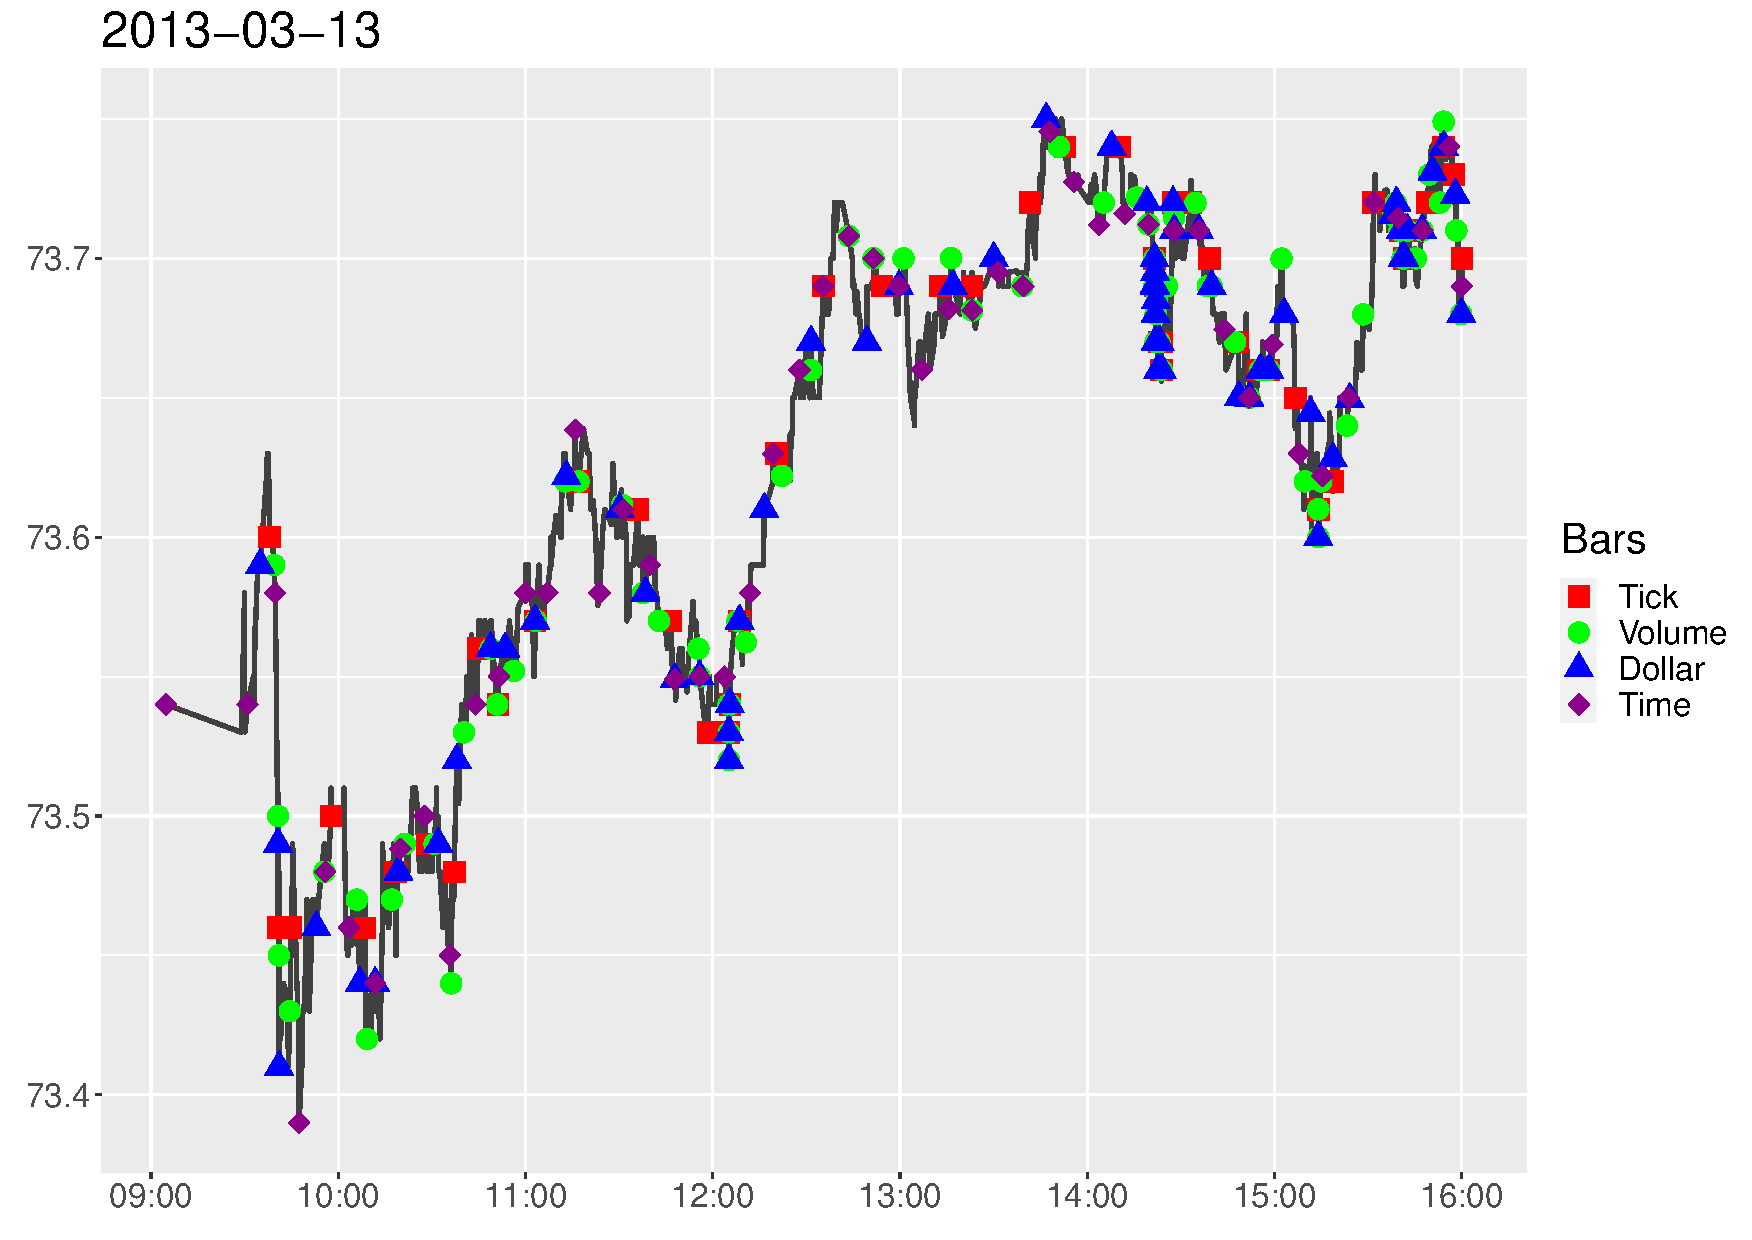
\includegraphics[scale=.25]{img/dataBars/sampling1}
	\end{subfigure}%
	\begin{subfigure}{.5\textwidth}
		\centering
		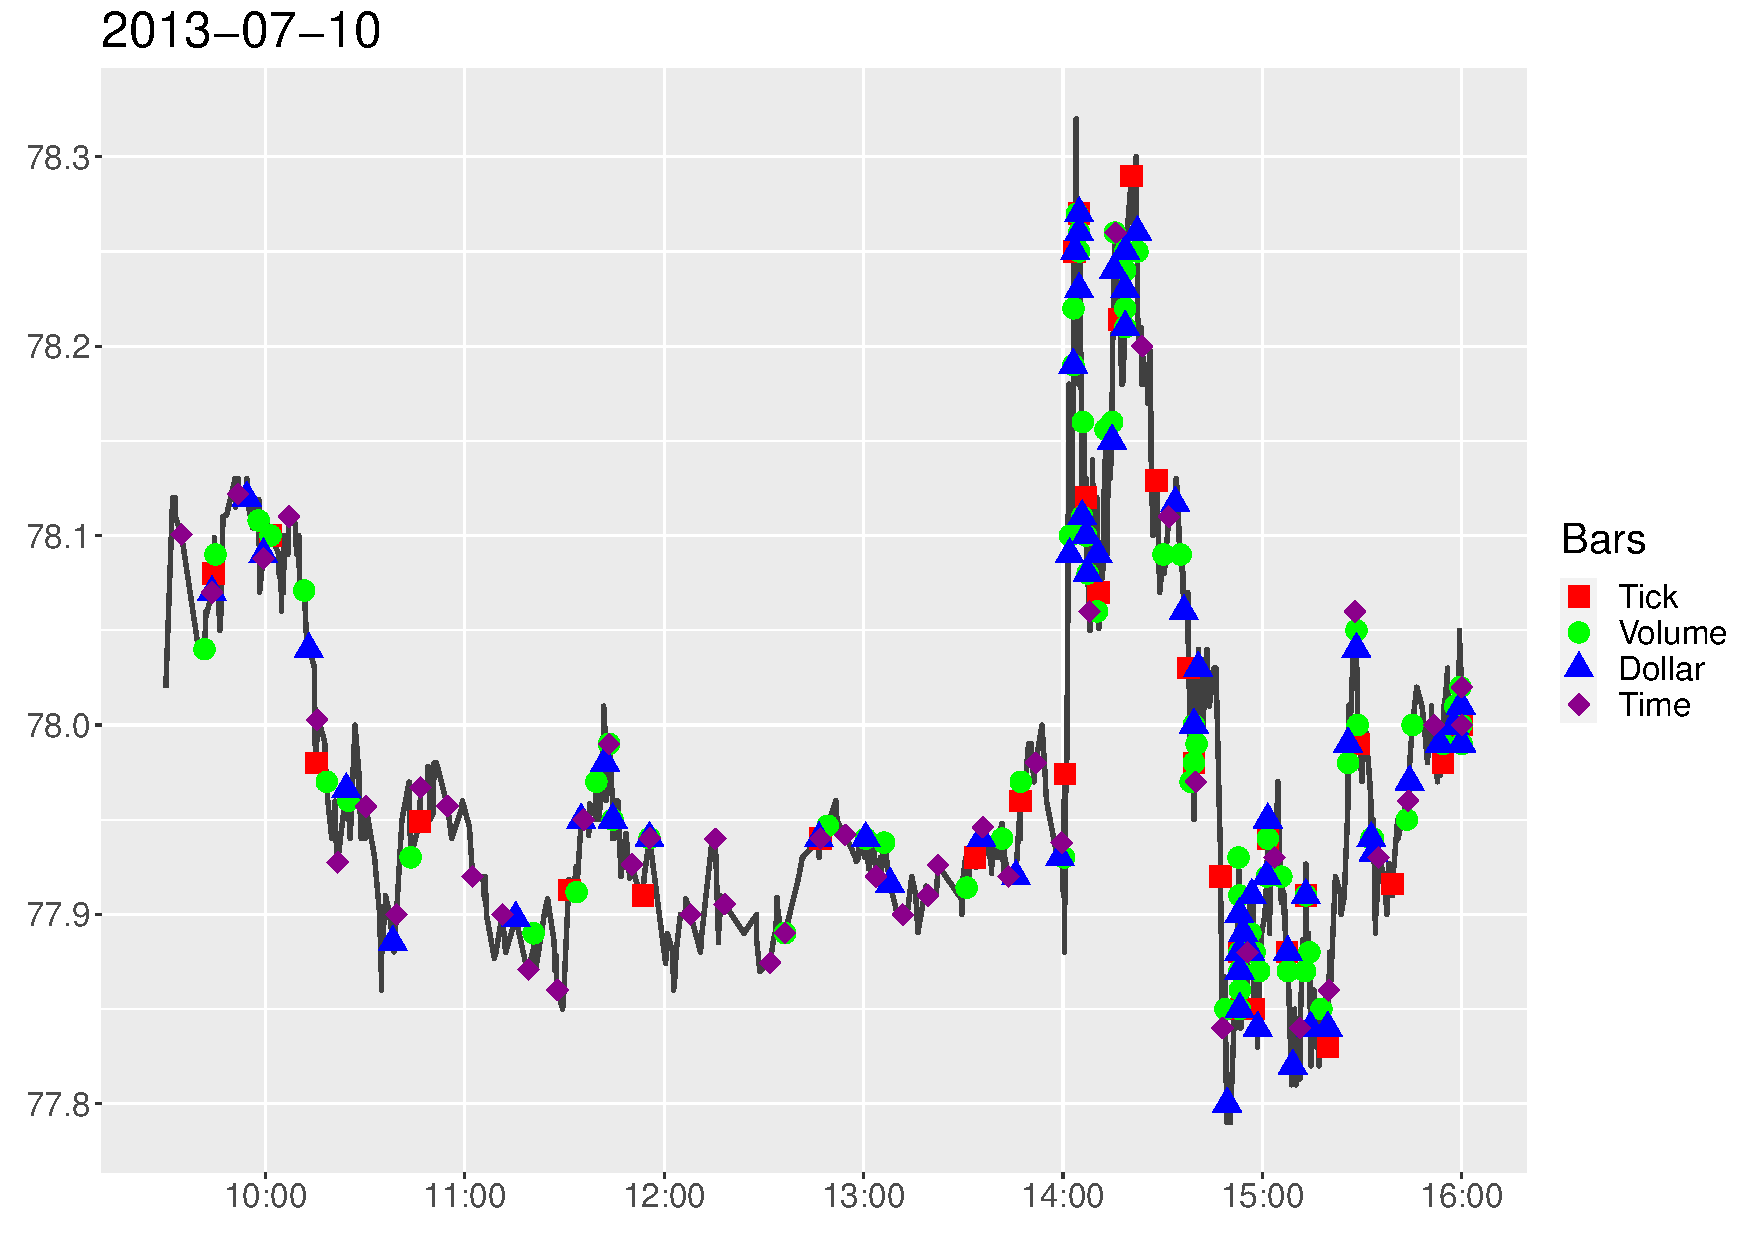
\includegraphics[scale=.25]{img/dataBars/sampling2}
	\end{subfigure}%

	\vspace{.4cm}

	\begin{subfigure}{\textwidth}
		\centering
		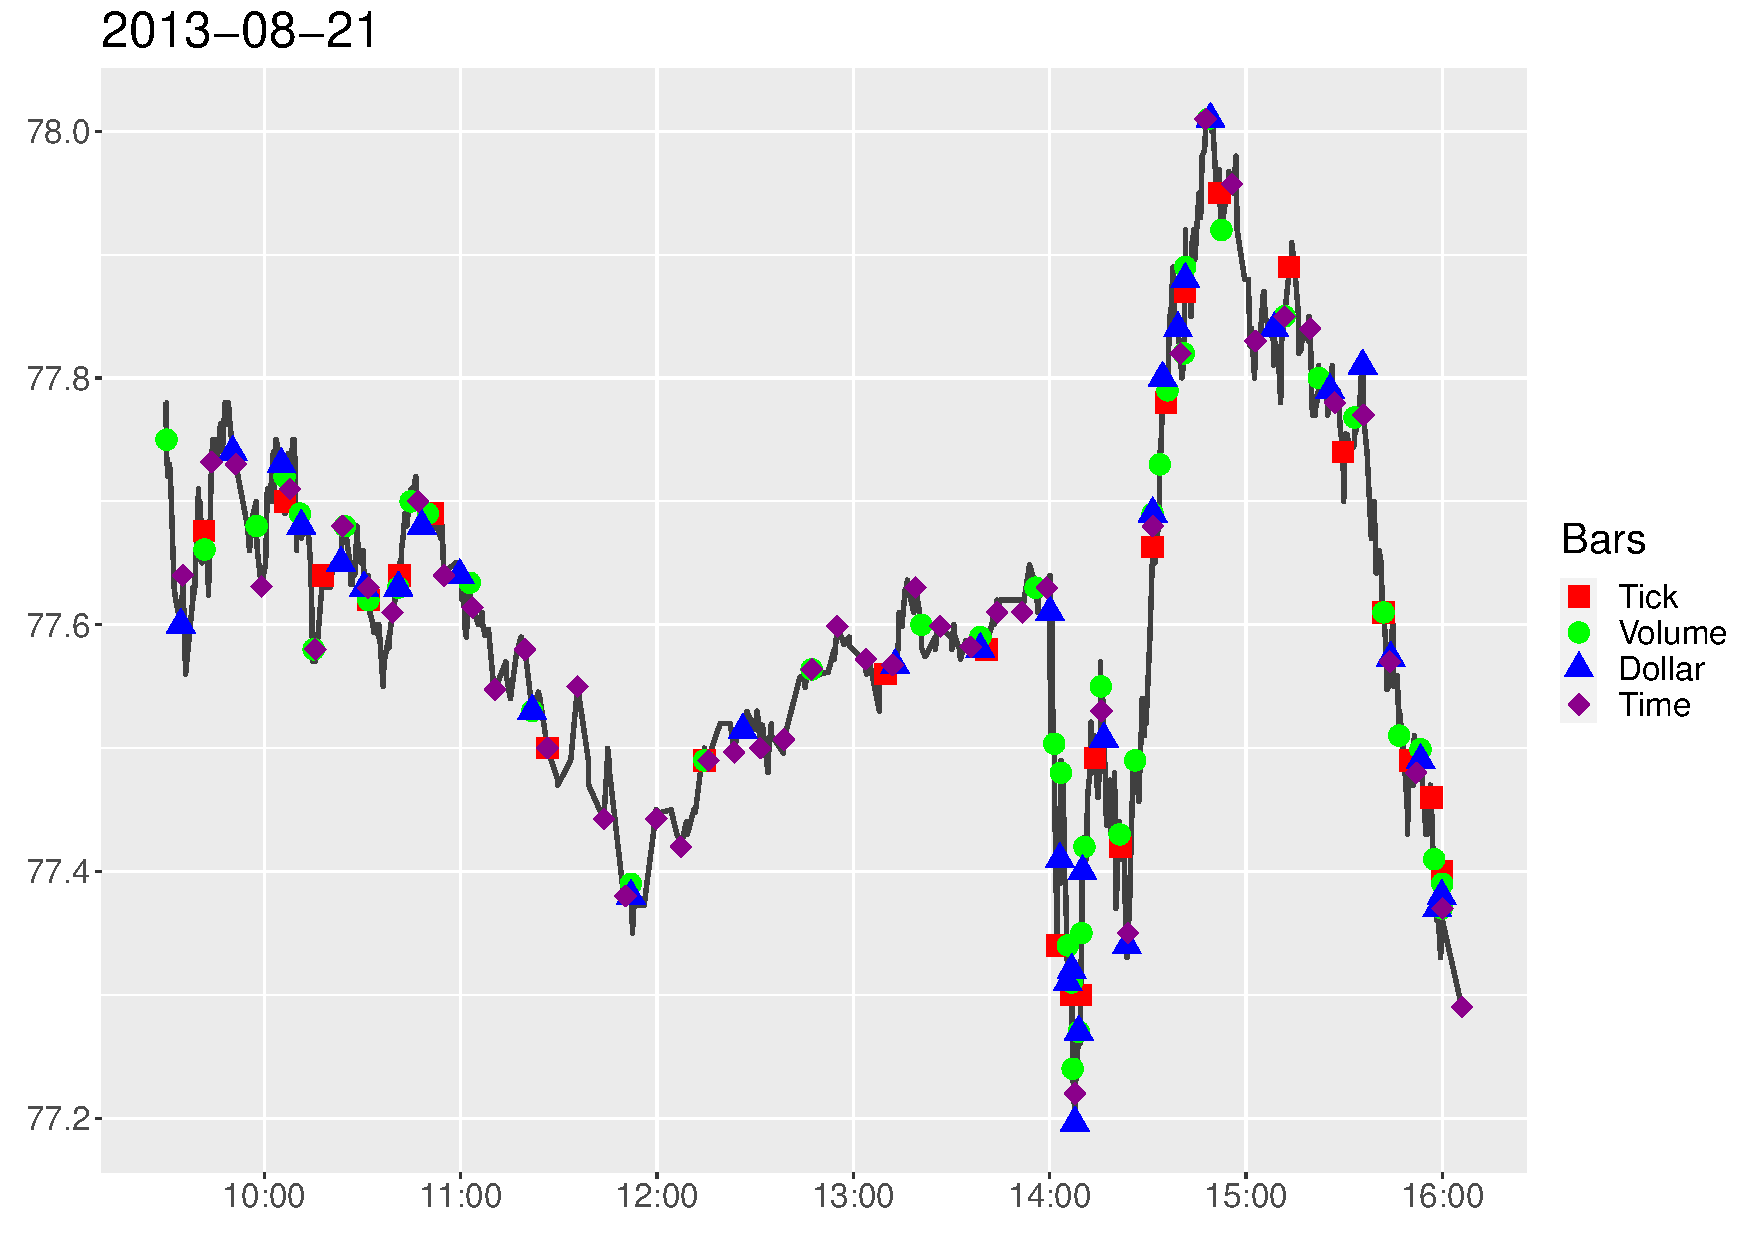
\includegraphics[scale=.25]{img/dataBars/sampling3}
	\end{subfigure}
	
	\caption{Tick, volume, dollar and time bars}
	\label{fig:dataBars}
\end{figure}

\begin{figure}[htbp]
	\centering
	
	\begin{subfigure}{\textwidth}
		\centering
		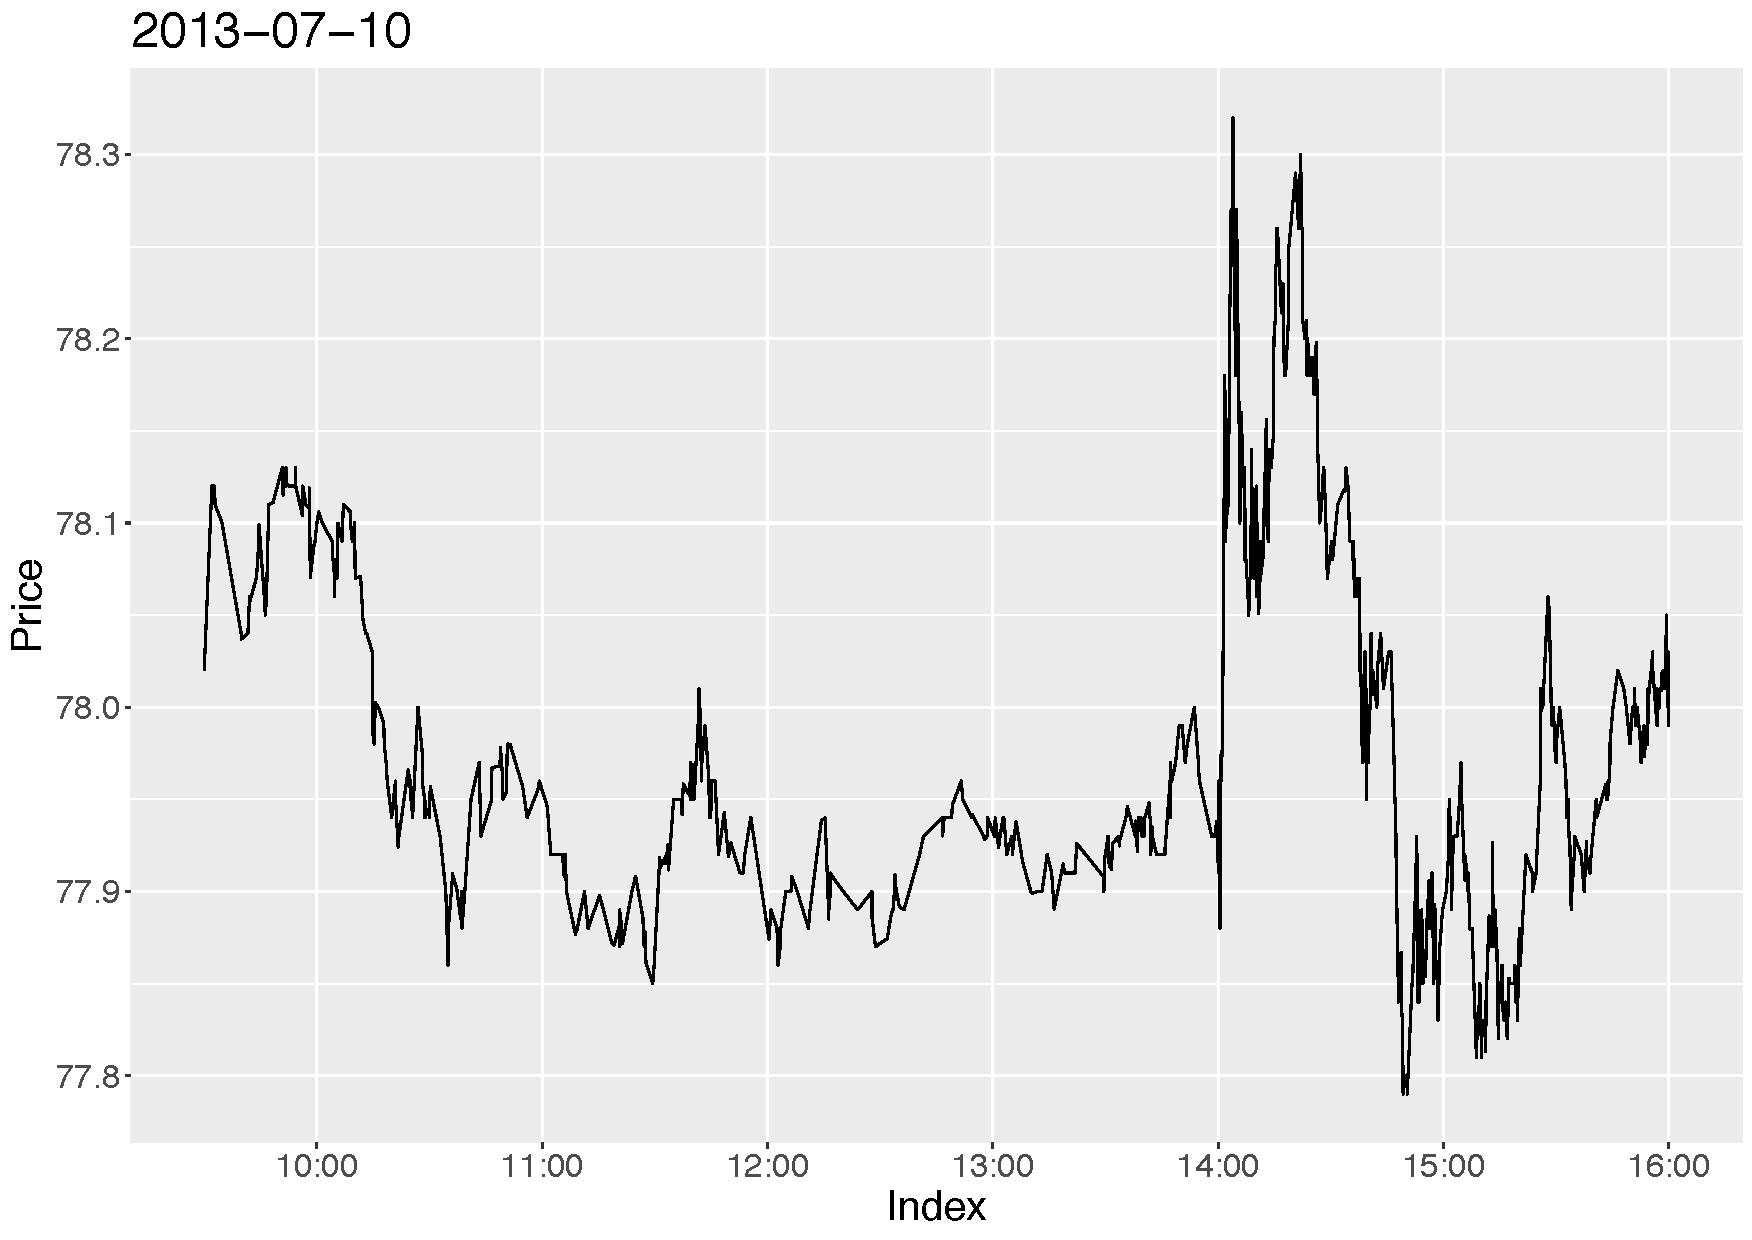
\includegraphics[scale=.5]{img/dataBars/regularZoom}
		\caption{Tick data}
	\end{subfigure}%
	
	\vspace{.4cm}
	
	\begin{subfigure}{.5\textwidth}
		\centering
		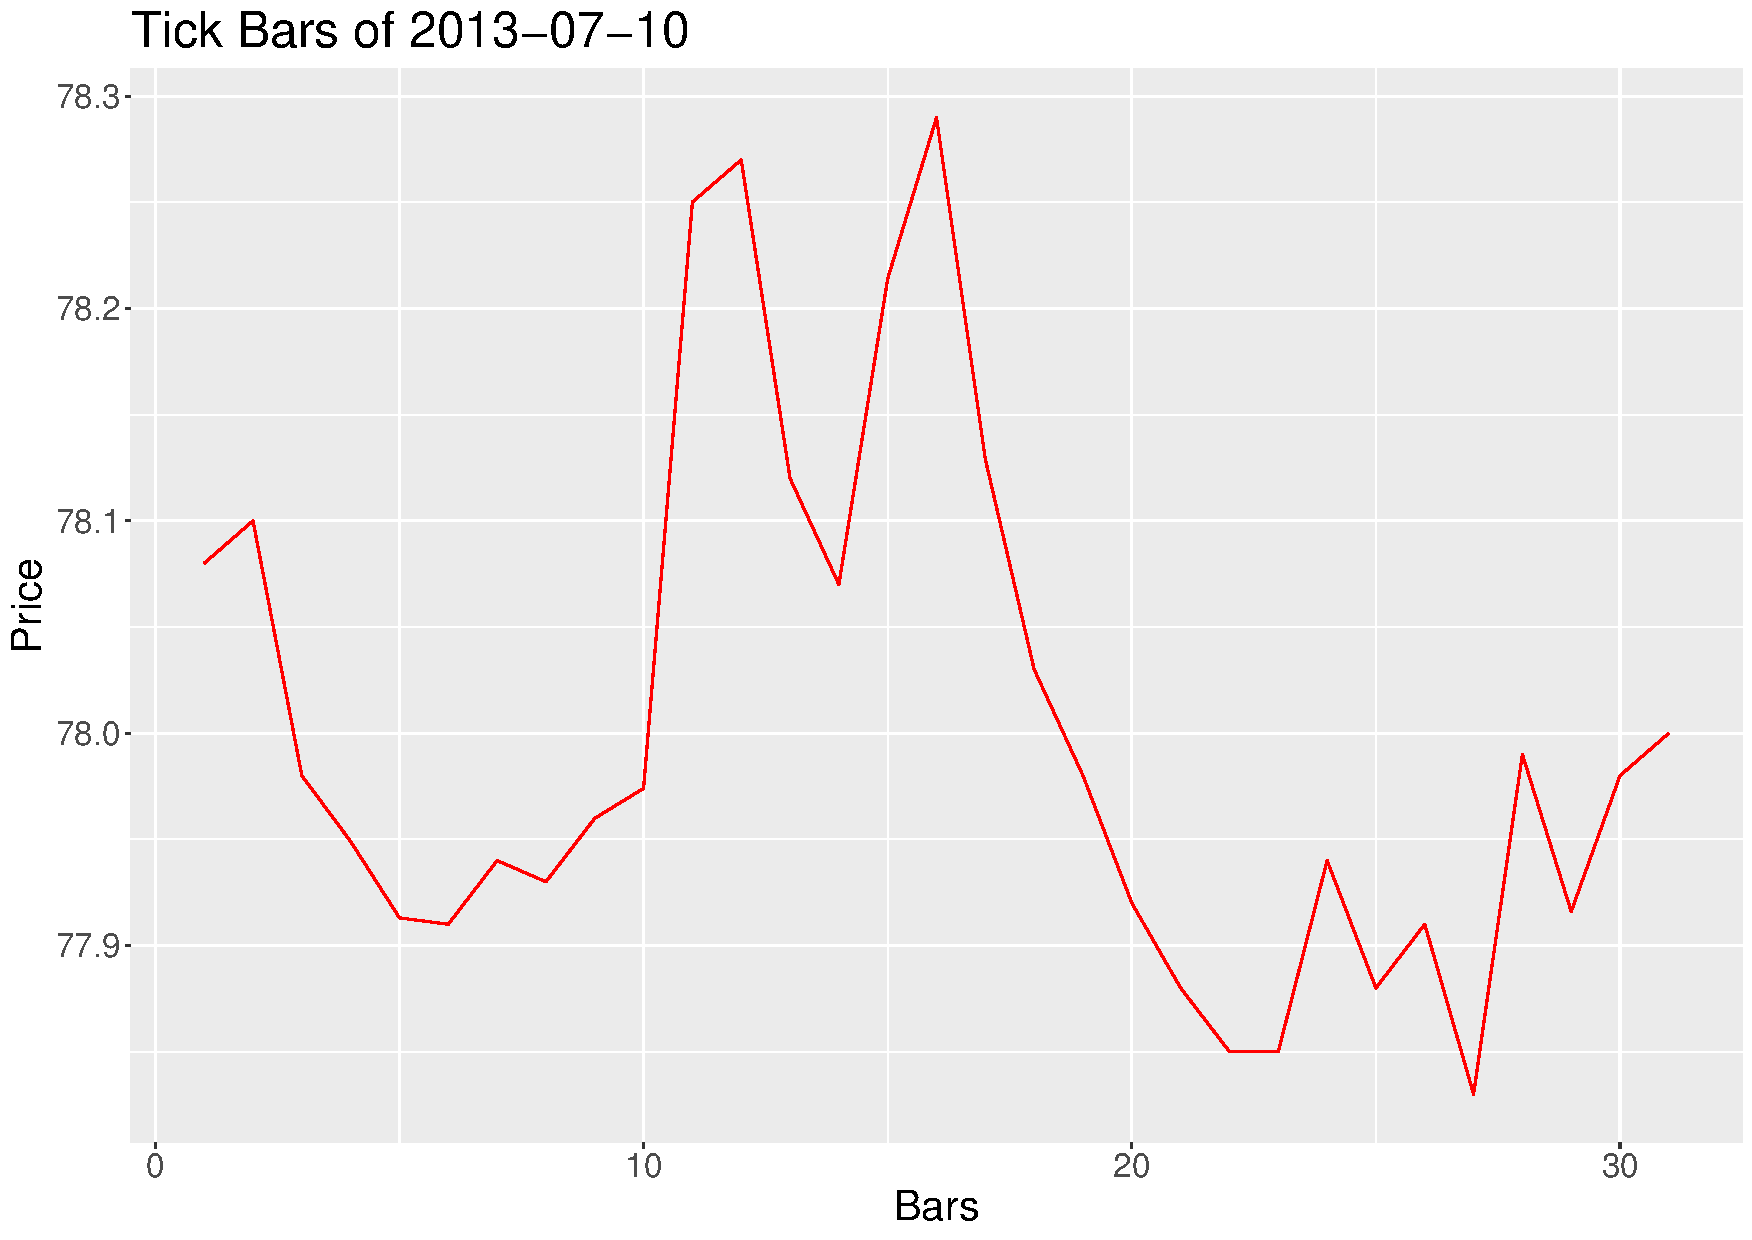
\includegraphics[scale=.25]{img/dataBars/tickZoom}
		\caption{Tick bars}
	\end{subfigure}%
	\begin{subfigure}{.5\textwidth}
		\centering
		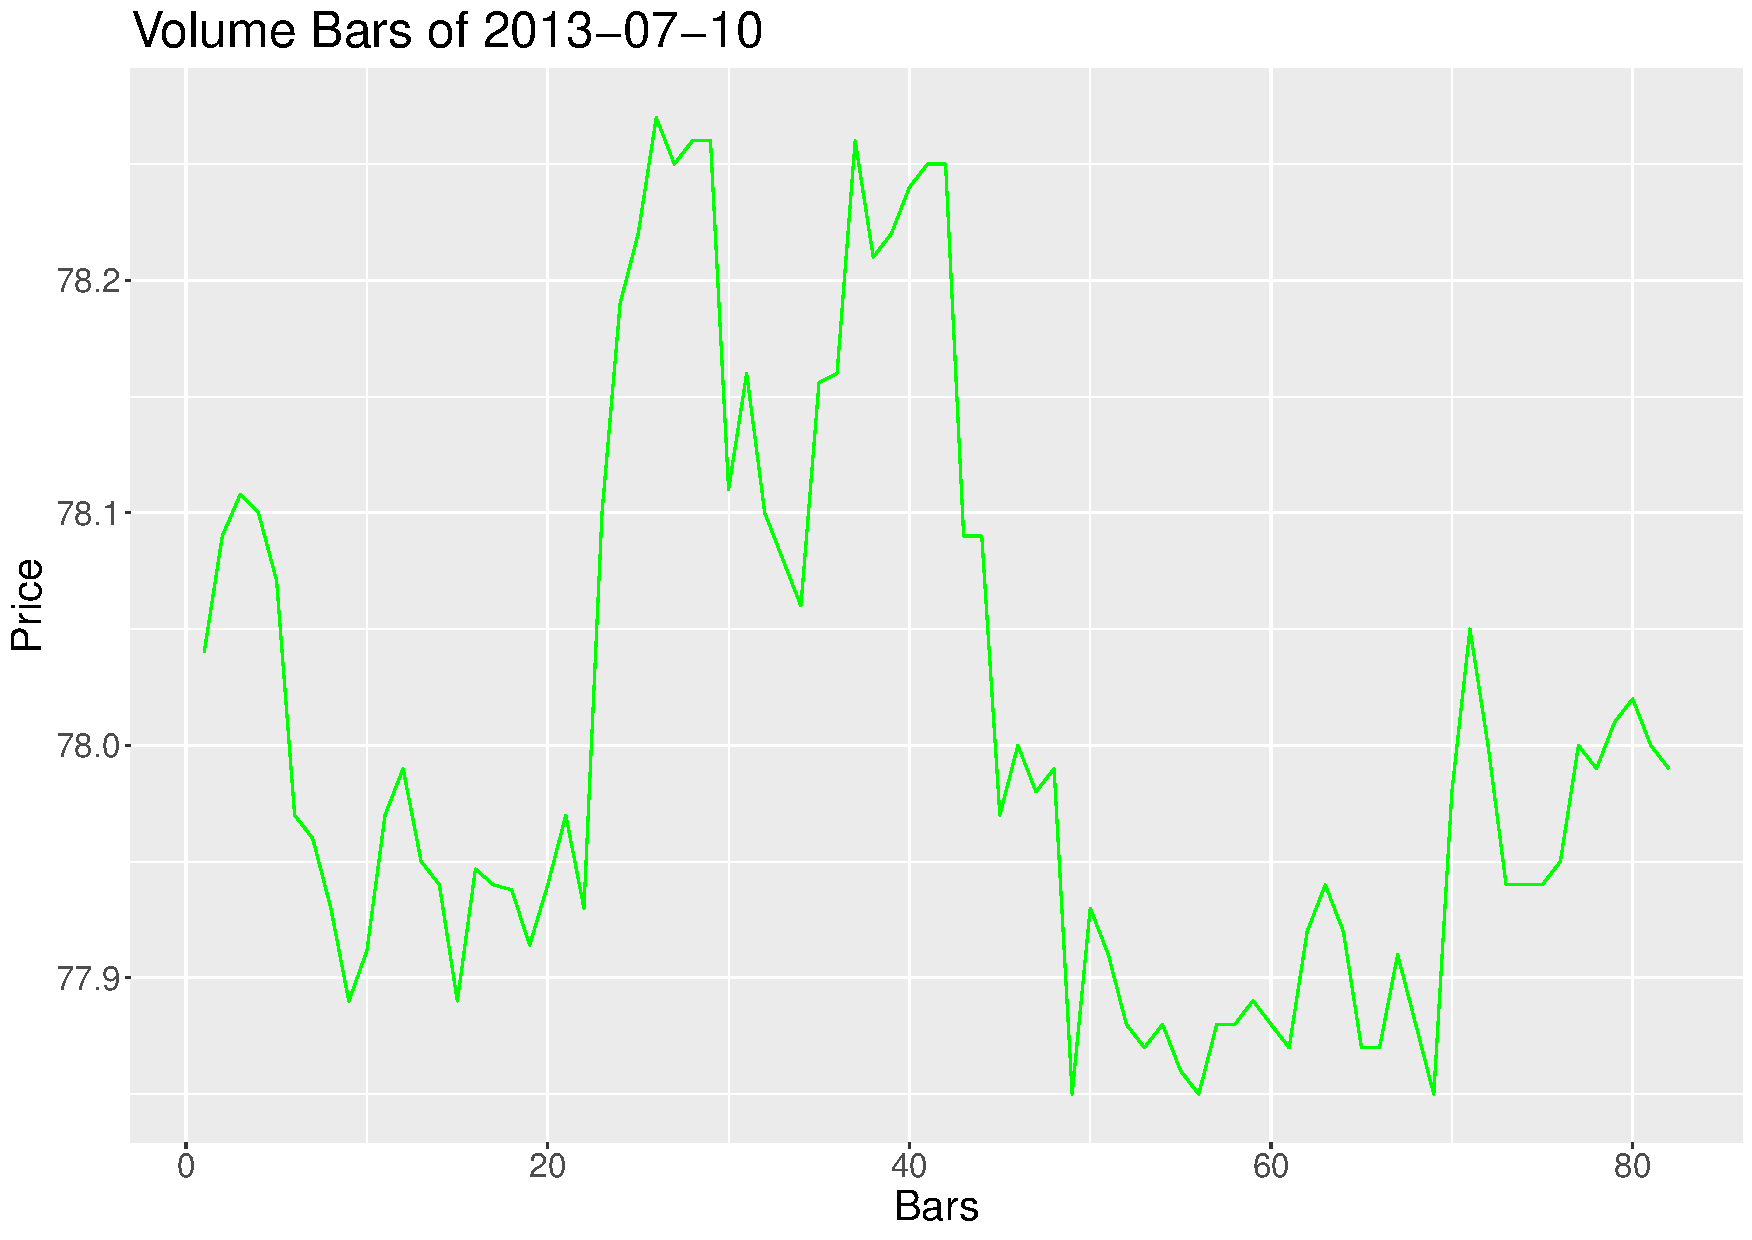
\includegraphics[scale=.25]{img/dataBars/volumeZoom}
		\caption{Volume bars}
	\end{subfigure}%

	\vspace{.4cm}

	\begin{subfigure}{.5\textwidth}
		\centering
		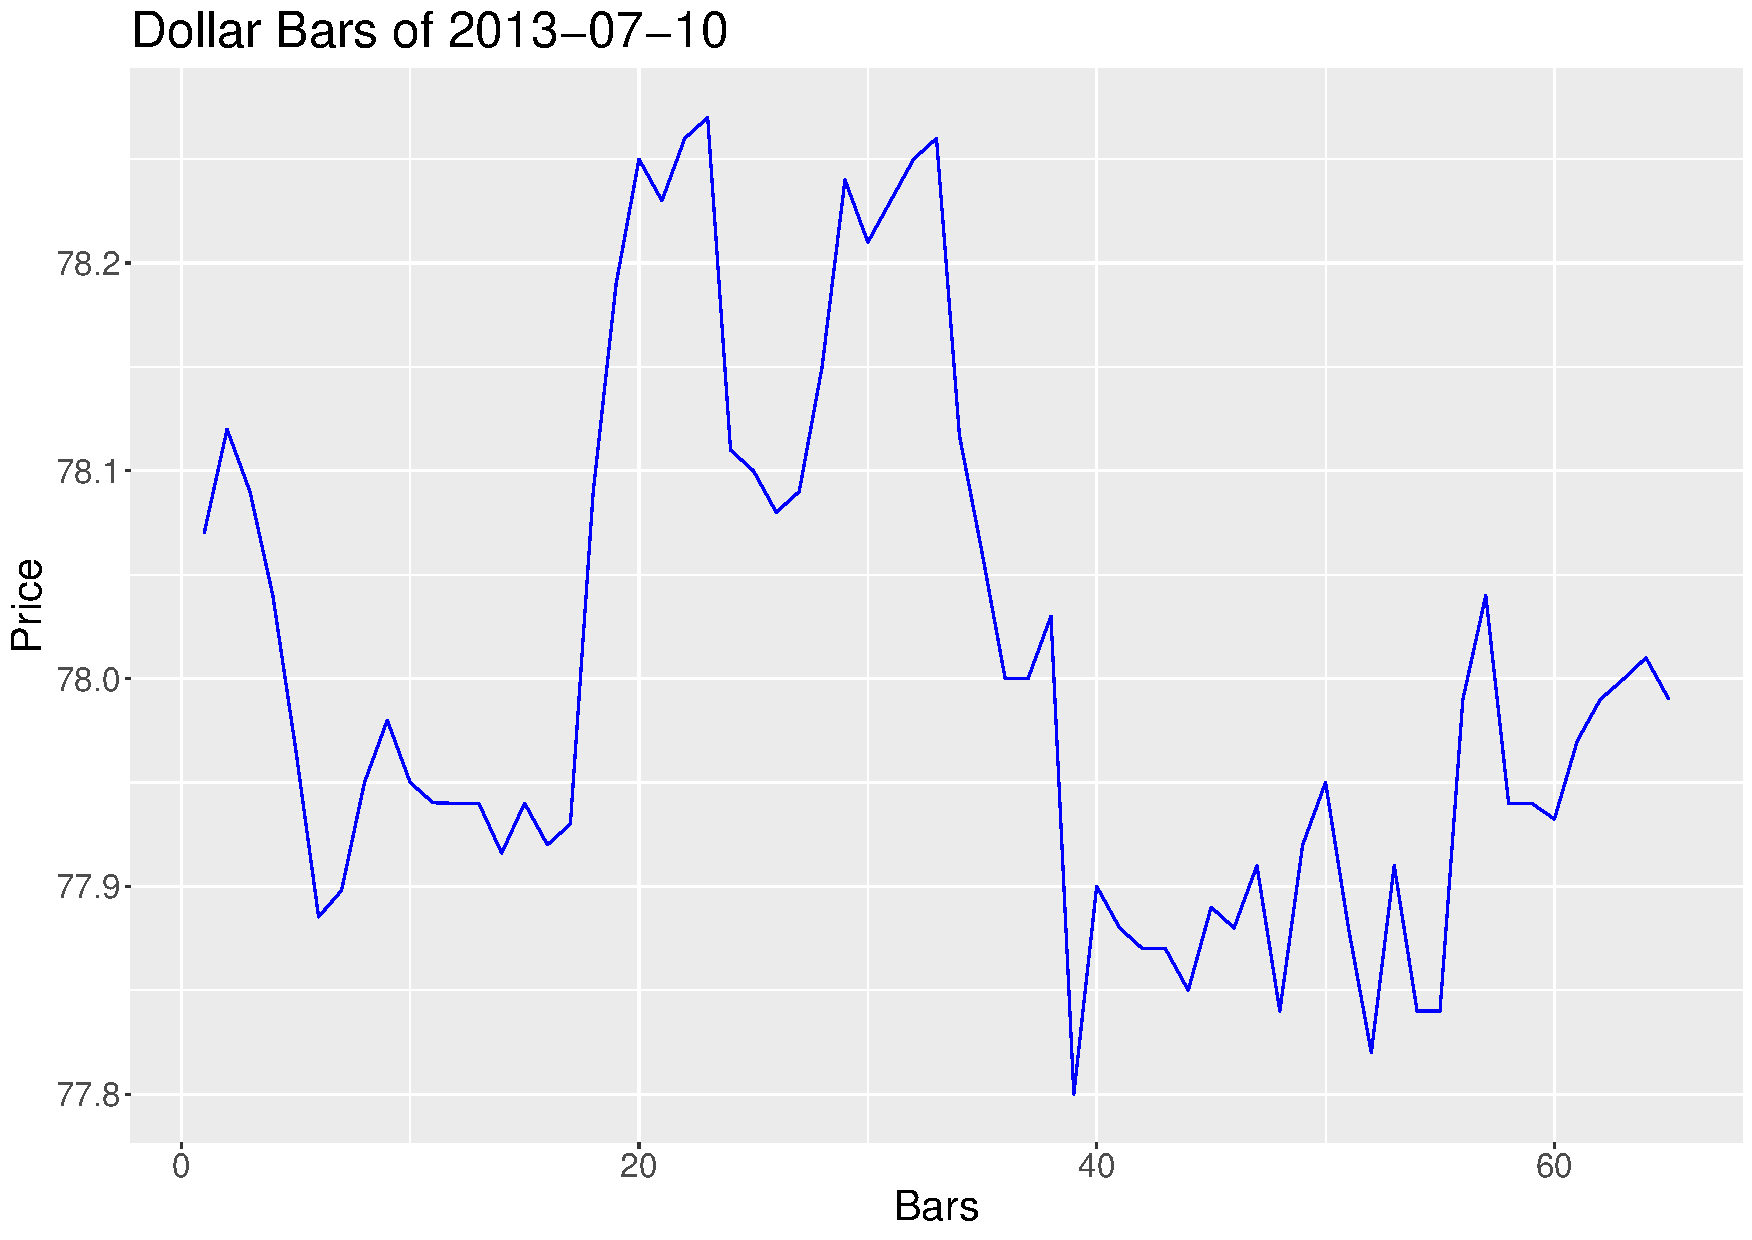
\includegraphics[scale=.25]{img/dataBars/dollarZoom}
		\caption{Dollar bars}
	\end{subfigure}%
	\begin{subfigure}{.5\textwidth}
		\centering
		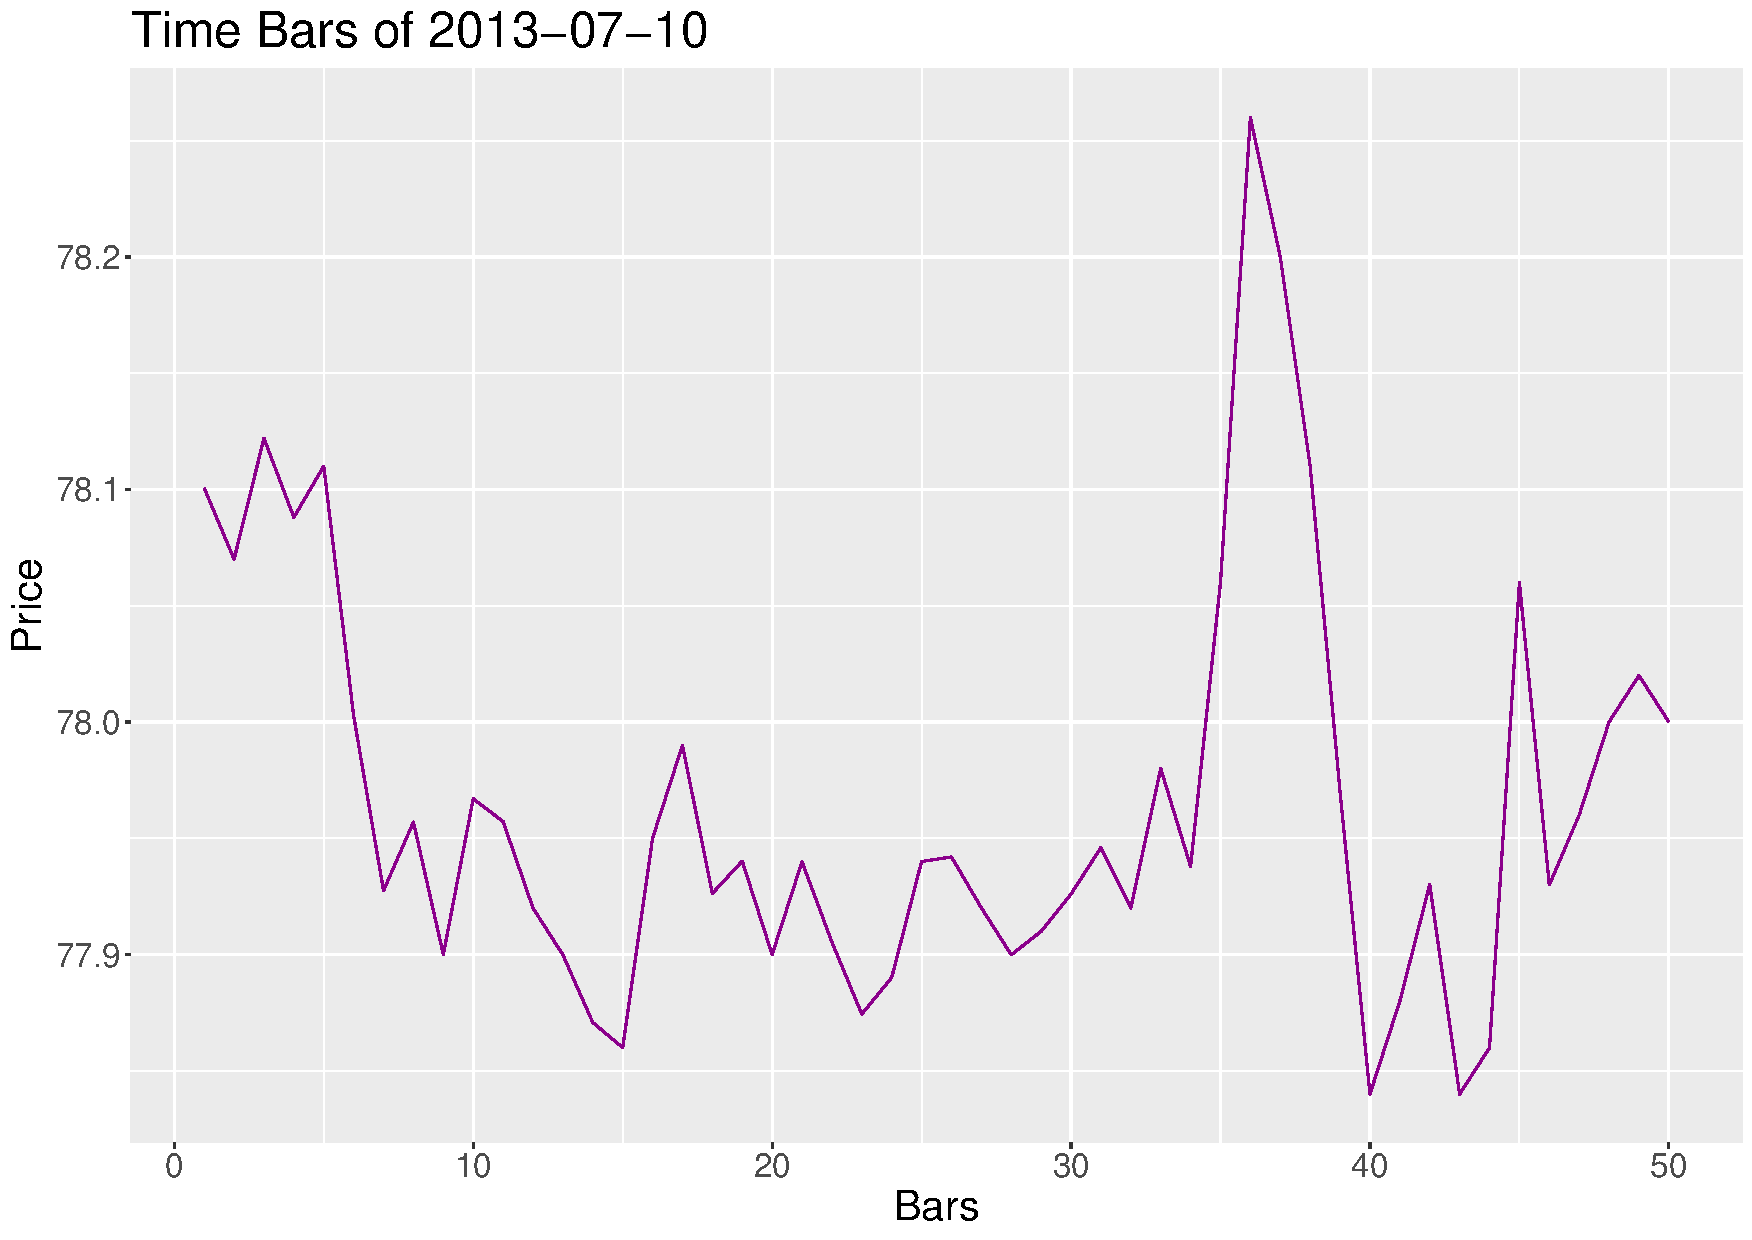
\includegraphics[scale=.25]{img/dataBars/timeZoom}
		\caption{Time bars}
	\end{subfigure}%
	
	\caption{Sampling of 2013-07-10 tick data via tick, volume, dollar and 
	time bars}
	\label{fig:intradayDeformed}
\end{figure}

\newpage

\section{Normality of log-returns}
\label{sec:normalLogRet}
Once the samples have been gathered, it is time to compute log-returns and 
analyze their distribution. López de Prado argues in~\cite{volumeClock} that 
the time transformation induced by data bars allows a partial recovery of 
Normality.\\

However, after normalizing data, i.e. transform it such that it has a 
mean of 0 and a standard deviation of 1, the pdfs are far from normal (see 
figures \ref{fig:pdfLogReturns} and \ref{fig:QQPlotsDataBars}). Even after 
plotting the pdf of a $N(\mu = 0, \sigma = 0.5)$, it can be seen that the 
pdfs of all of the bars considered are heavy tailed.

\begin{figure}[htbp]
	\centering
	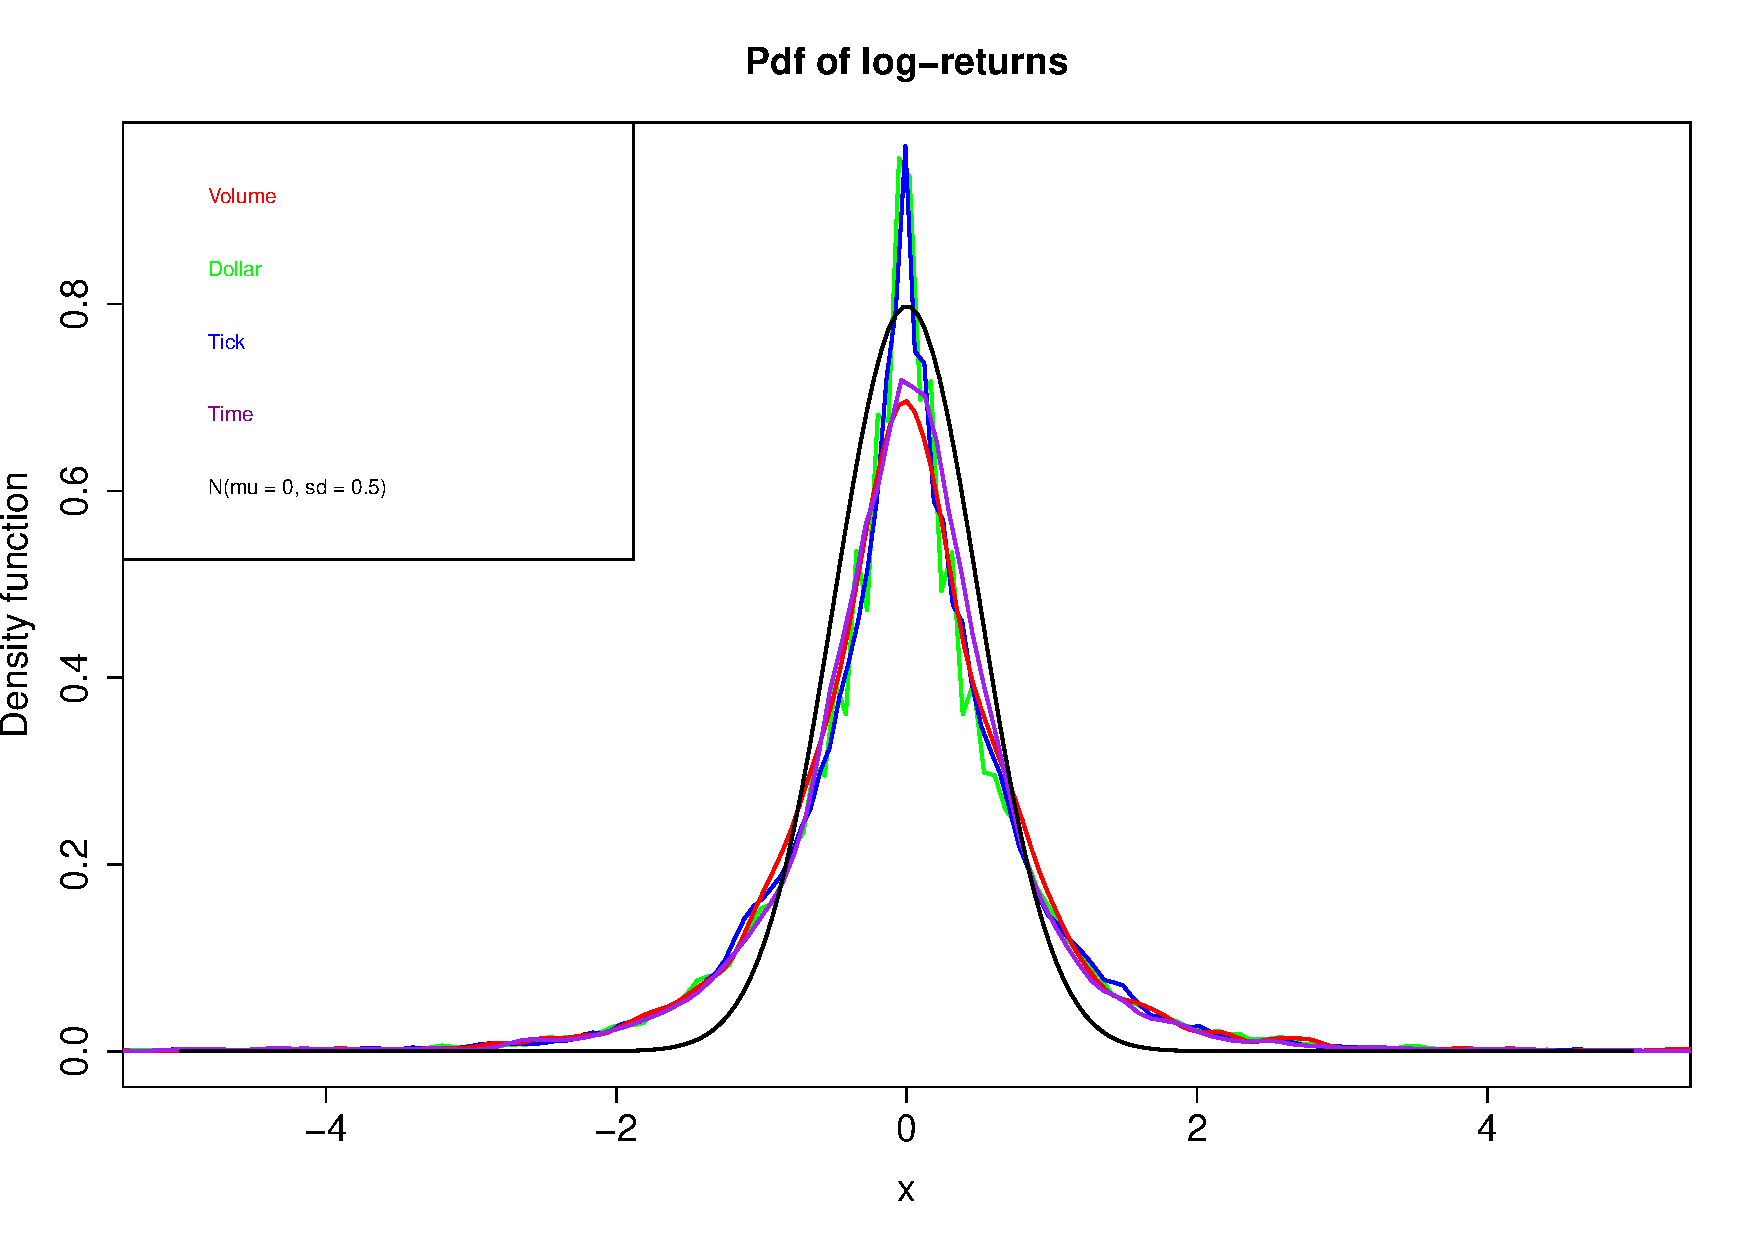
\includegraphics[scale=.35]{img/dataBars/pdfLogReturns}
	\caption{Fitted pdf of log-returns from data bars}
	\label{fig:pdfLogReturns}
\end{figure}

As a last comment on normality, note that in figure 
\ref{fig:QQPlotsDataBars} the QQ Plots of tick, volume and dollar bars have 
more pronounced tails than time bars. This is attributed to oversampling 
periods of high volatility, which by definition imply drastic changes in 
prices.

\begin{figure}[htbp]
	\centering

	\begin{subfigure}{.5\textwidth}
		\centering
		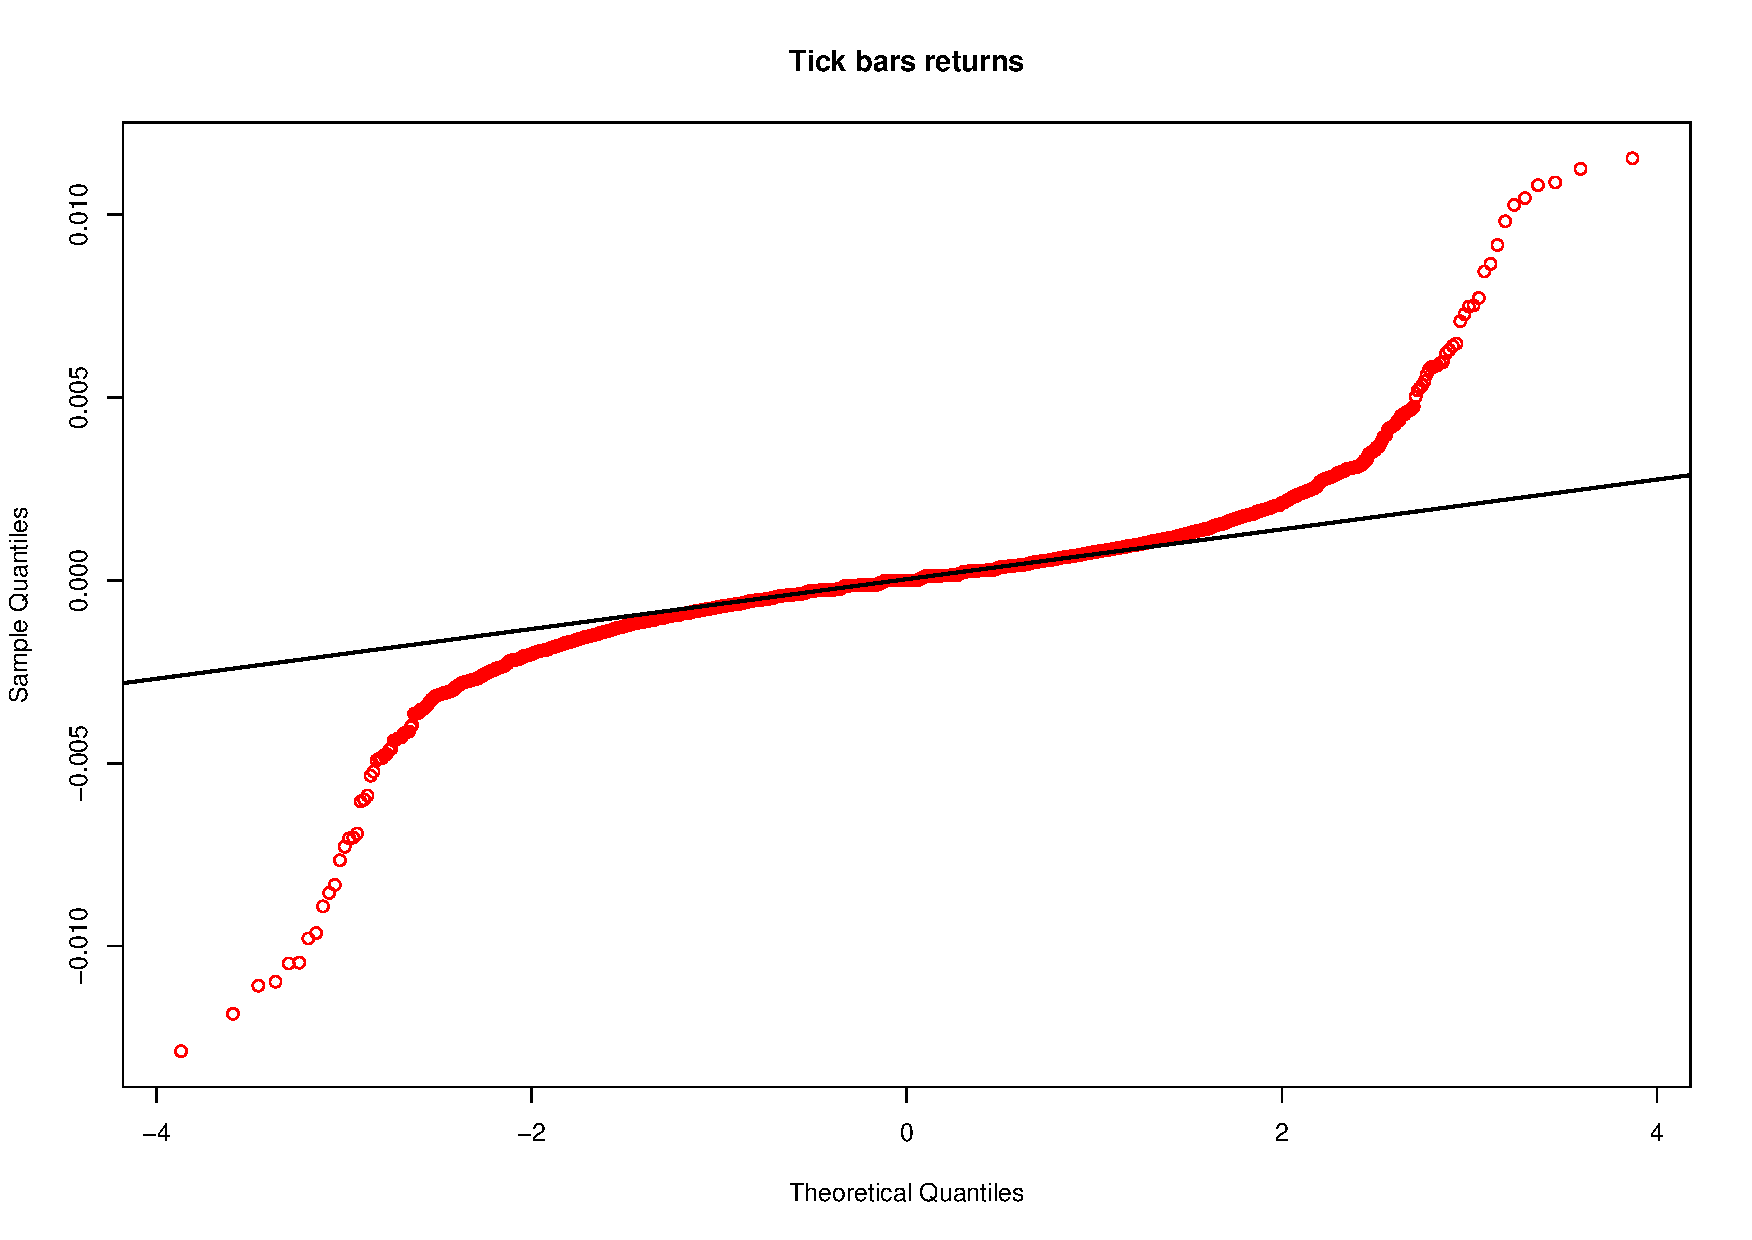
\includegraphics[scale=.25]{img/dataBars/tickQQPlot}
		\caption{Tick bars}
	\end{subfigure}%
	\begin{subfigure}{.5\textwidth}
		\centering
		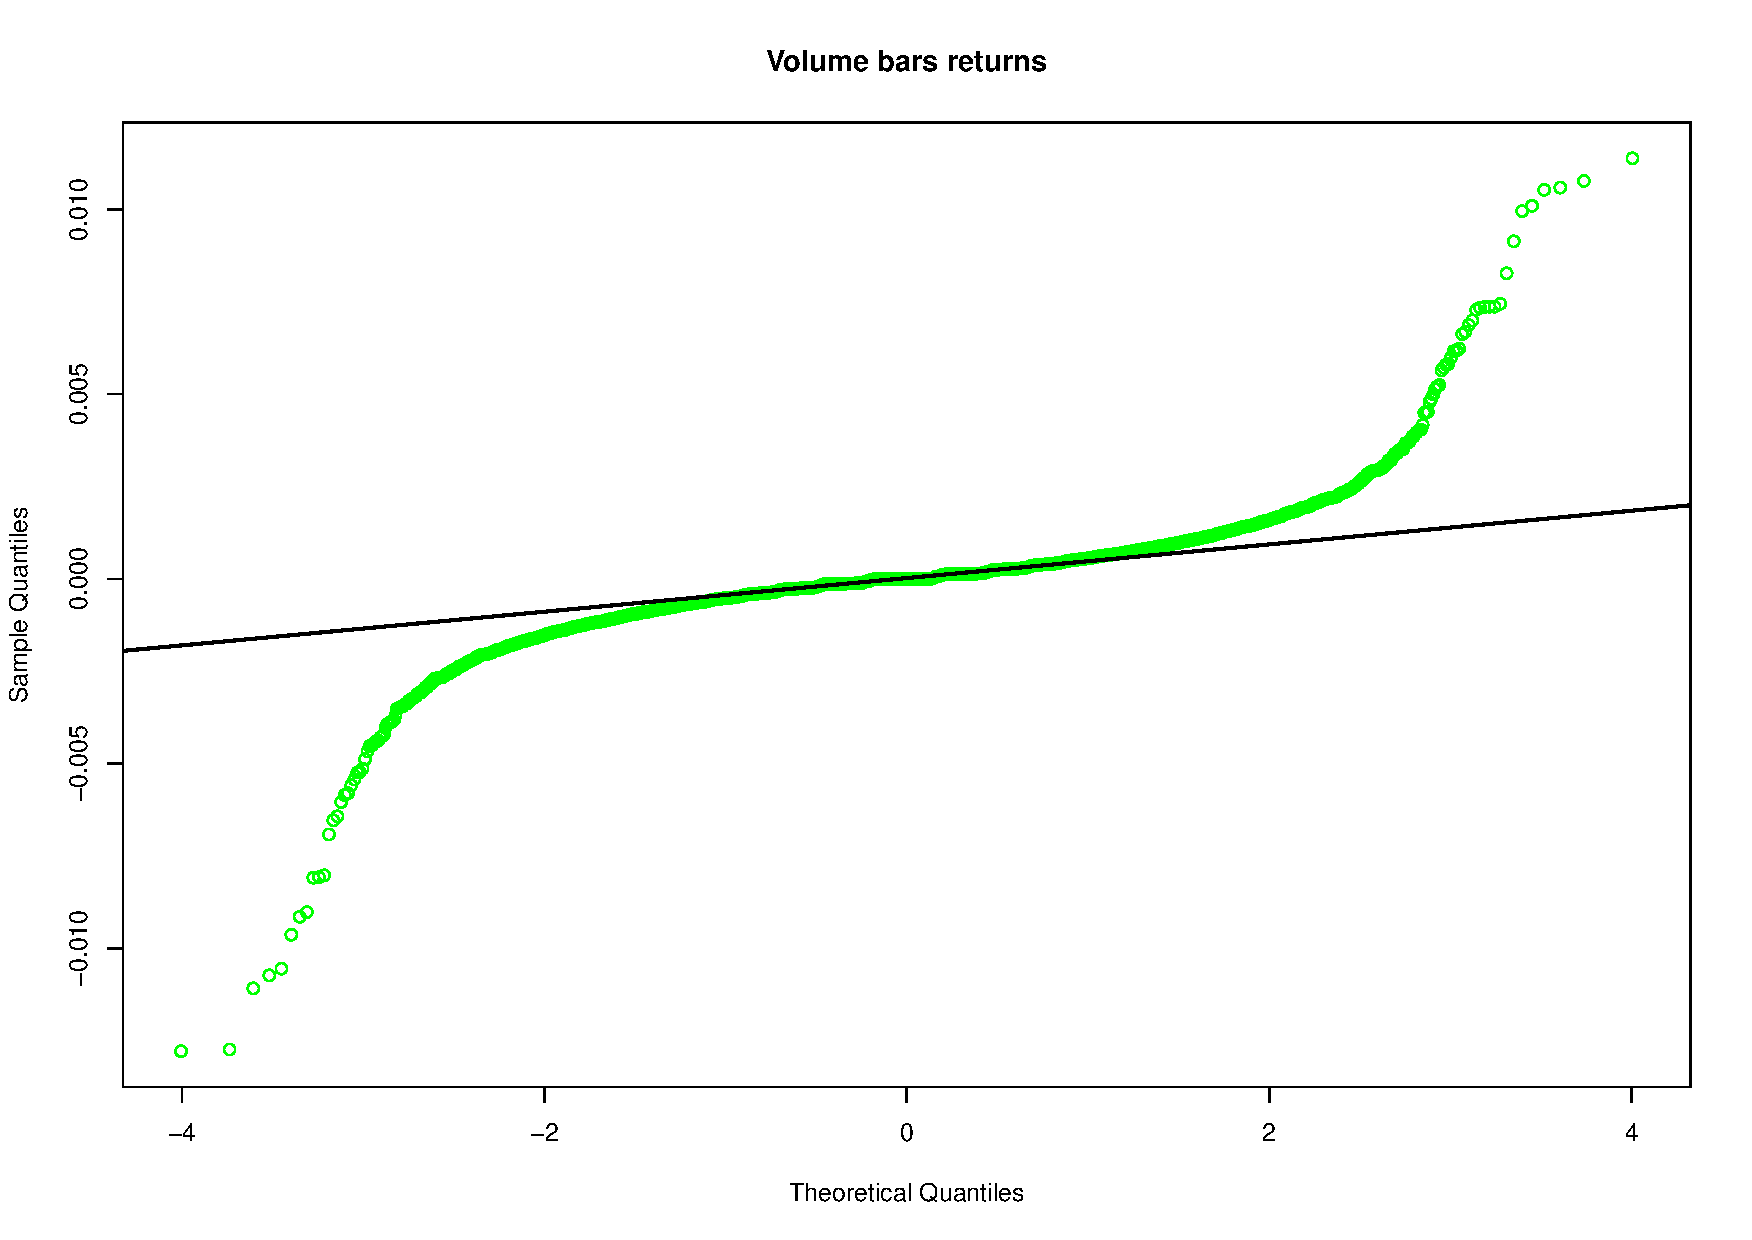
\includegraphics[scale=.25]{img/dataBars/volumeQQPlot}
		\caption{Volume bars}
	\end{subfigure}%

	\vspace{.4cm}

	\begin{subfigure}{.5\textwidth}
		\centering
		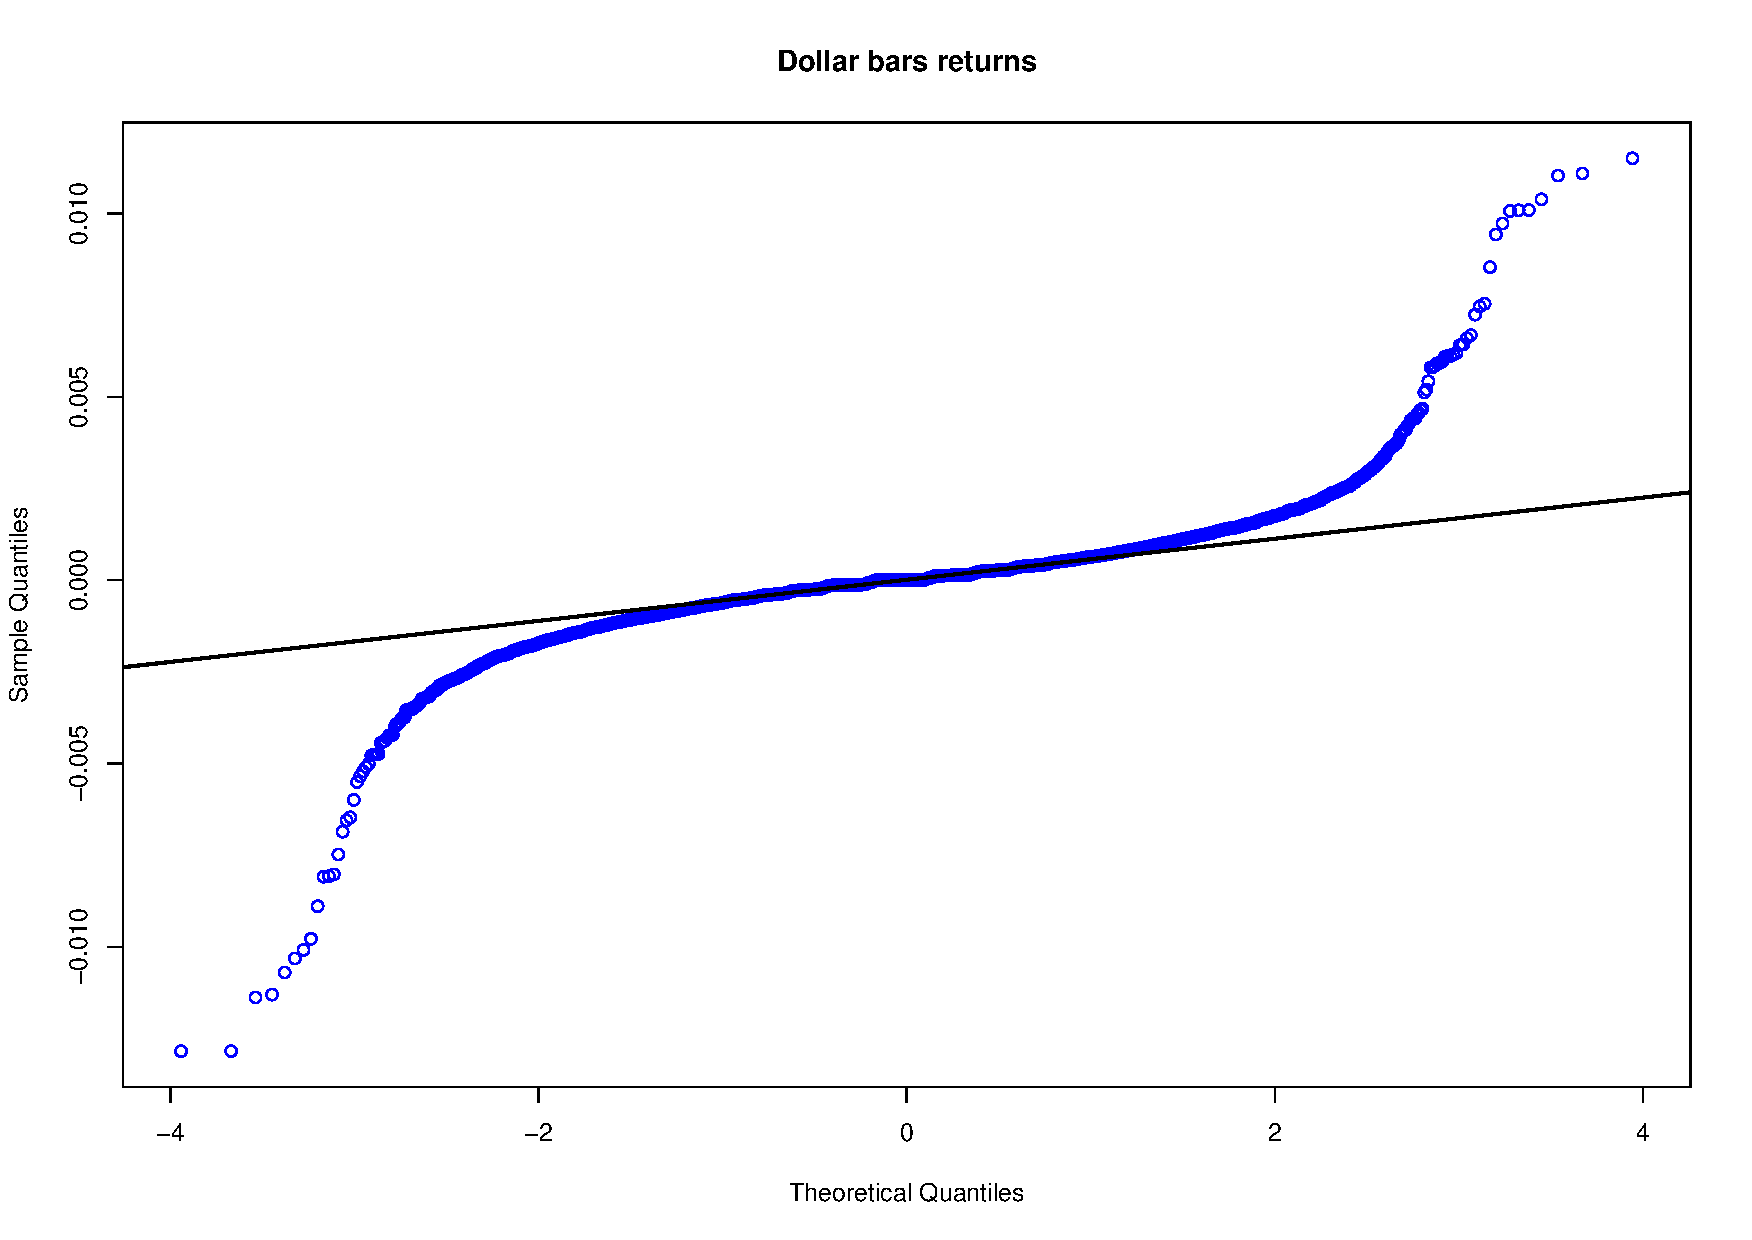
\includegraphics[scale=.25]{img/dataBars/dollarQQPlot}
		\caption{Dollar bars}
	\end{subfigure}%
	\begin{subfigure}{.5\textwidth}
		\centering
		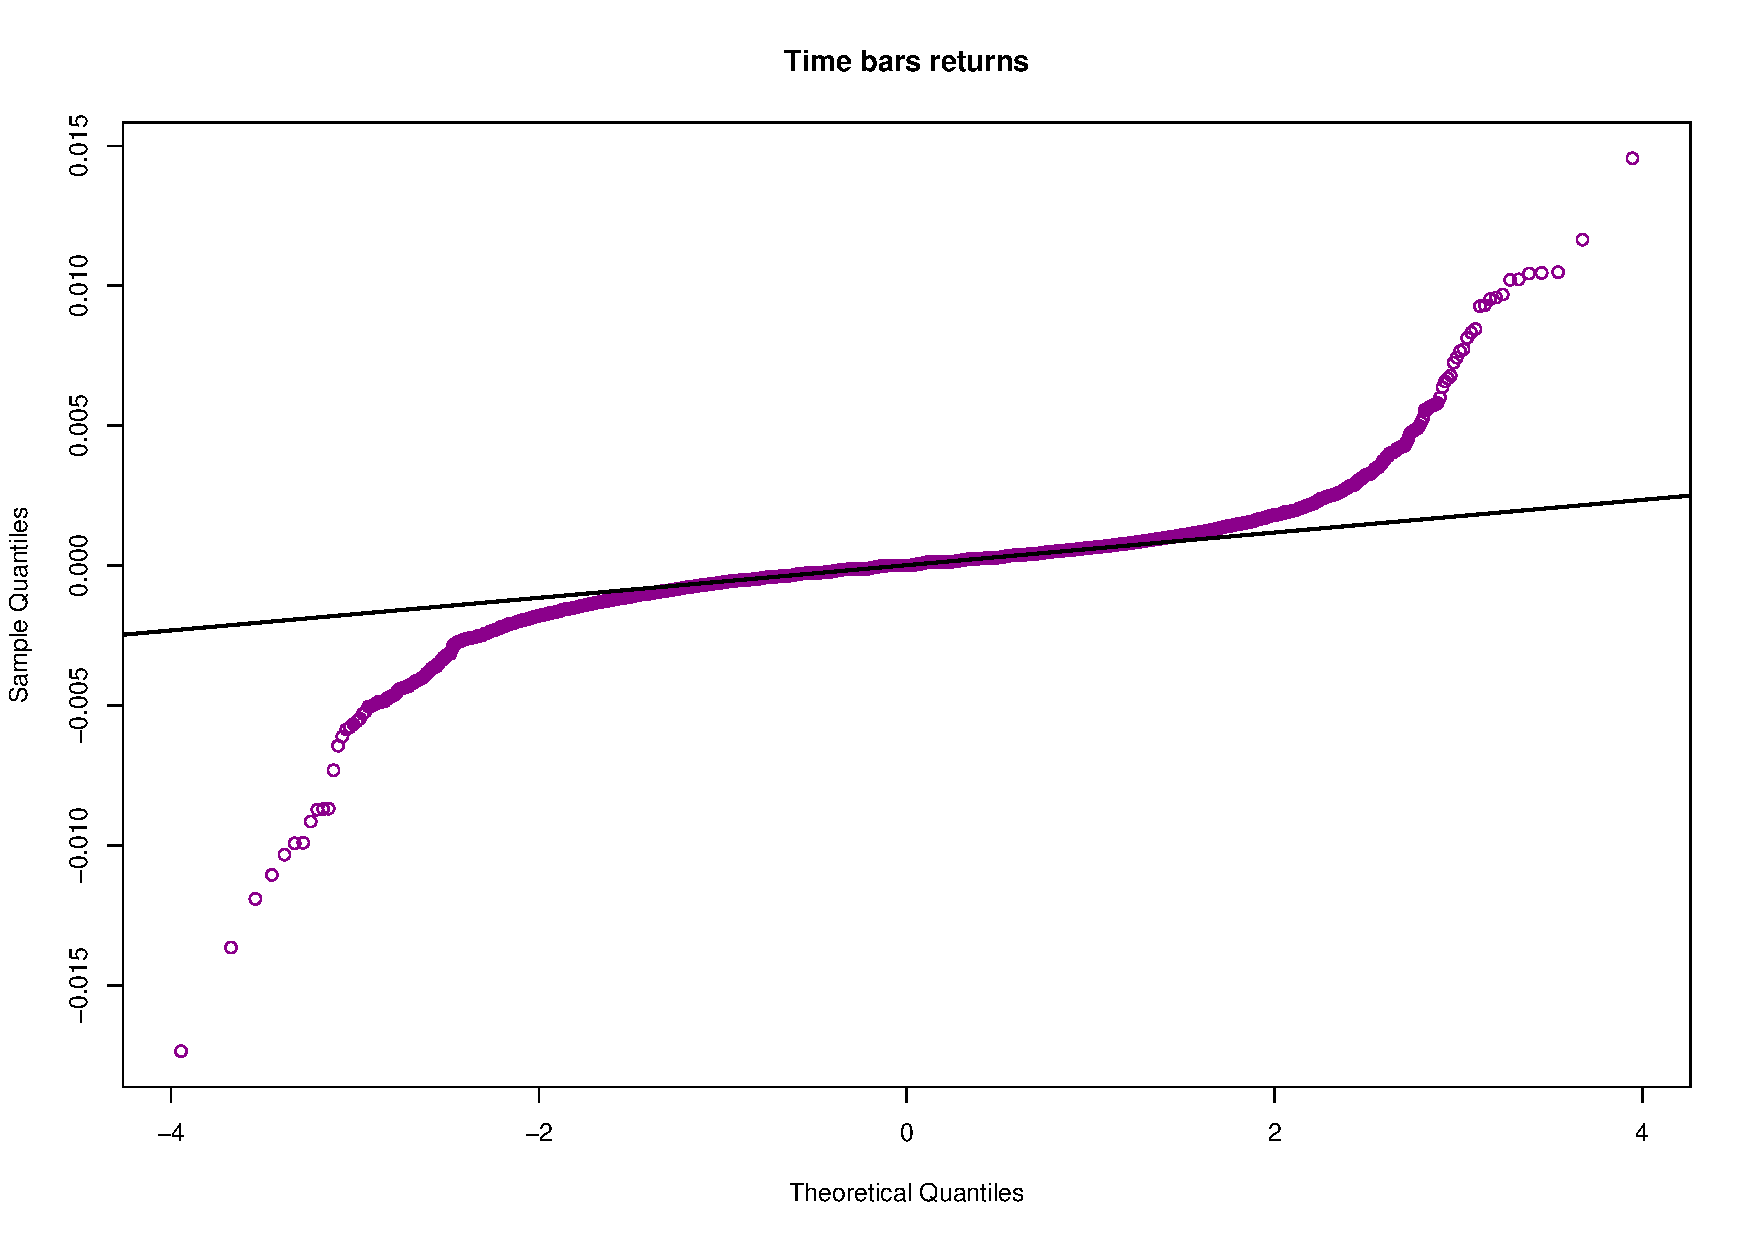
\includegraphics[scale=.25]{img/dataBars/timeQQPlot}
		\caption{Time bars}
	\end{subfigure}%
	
	\caption{QQ Plots of data bars}
	\label{fig:QQPlotsDataBars}
\end{figure}

\newpage

\section{Statistical analysis of bars}

With the aim of understanding better the behavior of data bars some 
parameters have been calculated and presented in table 
\ref{tab:statAnalysisDataBars}, giving rise to the following remarks:

\begin{itemize}
	\item Regarding $\text{ACF}_1$, the auto correlation function of lag 1, 
	time bars are the only type of bars that have a statistically 
	significant one.
	
	\item $\text{Var}[\widetilde{\sigma}^2]$ is the variance of 
	$\widetilde{\sigma}^2$, where the latter is the square of monthly 
	volatility. Therefore, a small variance will mean that volatility tends 
	to stay fairly constant month over month. This is what happened with 
	volume bars, whose variation of monthly volatility is the lowest.
	
	\item $\bar{n}^{\text{weekly}}$, the average number of bars in a week 
	shows that tick bars have the fewest, dollar and time bars really 
	similar numbers, and volume bars having the most.
	
	\item $\text{SD}[n^{\text{weekly}}]$, the standard deviation of the 
	number of weekly bars, shows that time bars are the most stable ones. 
	This should not be a surprise because being equally time spaced makes 
	them deterministic, with the only variability introduced via weeks with 
	holidays. Apart from that, tick and dollar bars follow along and volume 
	bars are the ones that display the most variability.
\end{itemize}

\begin{table}[htbp]
\caption{Statistical analysis of bars}
\label{tab:statAnalysisDataBars}
\centering
\begin{tabular}{ |C{3cm}|C{3cm}|C{3cm}|C{3cm}|C{3cm}| }
	\hline
	 				& Tick & Volume & Dollar & Time\\
	\hline
	%Jarque-Bera Statistic & 191,732.4 & 838,289.1 & 512,942.7 & 696,297.4\\
	$\text{ACF}_1$ & -0.01090561 & -0.01225259 & -0.01482256 & 
	-0.06833088\\
	$\text{Var}[\widetilde{\sigma}^2]$ & $2.936431 \cdot 10^{-13}$ &   
	$7.139122 \cdot 10^{-14}$ & $1.054108 \cdot 10^{-13}$ & 
	$1.618769 \cdot 10^{-13}$\\
	$\bar{n}^{\text{weekly}}$ & 173.1509 & 303.1698 & 233.9245 & 237.3962\\
	$\text{SD}[n^{\text{weekly}}]$ & 63.95744 & 101.94866 & 73.20699 
	& 31.19069\\
	\hline
\end{tabular}
\end{table}

To complement the information given in table \ref{tab:statAnalysisDataBars}, 
figure \ref{fig:weeklyBarCounts} shows the normalized (to a [0,1] interval) 
number of weekly bars.

\begin{figure}[htbp]
	\centering
	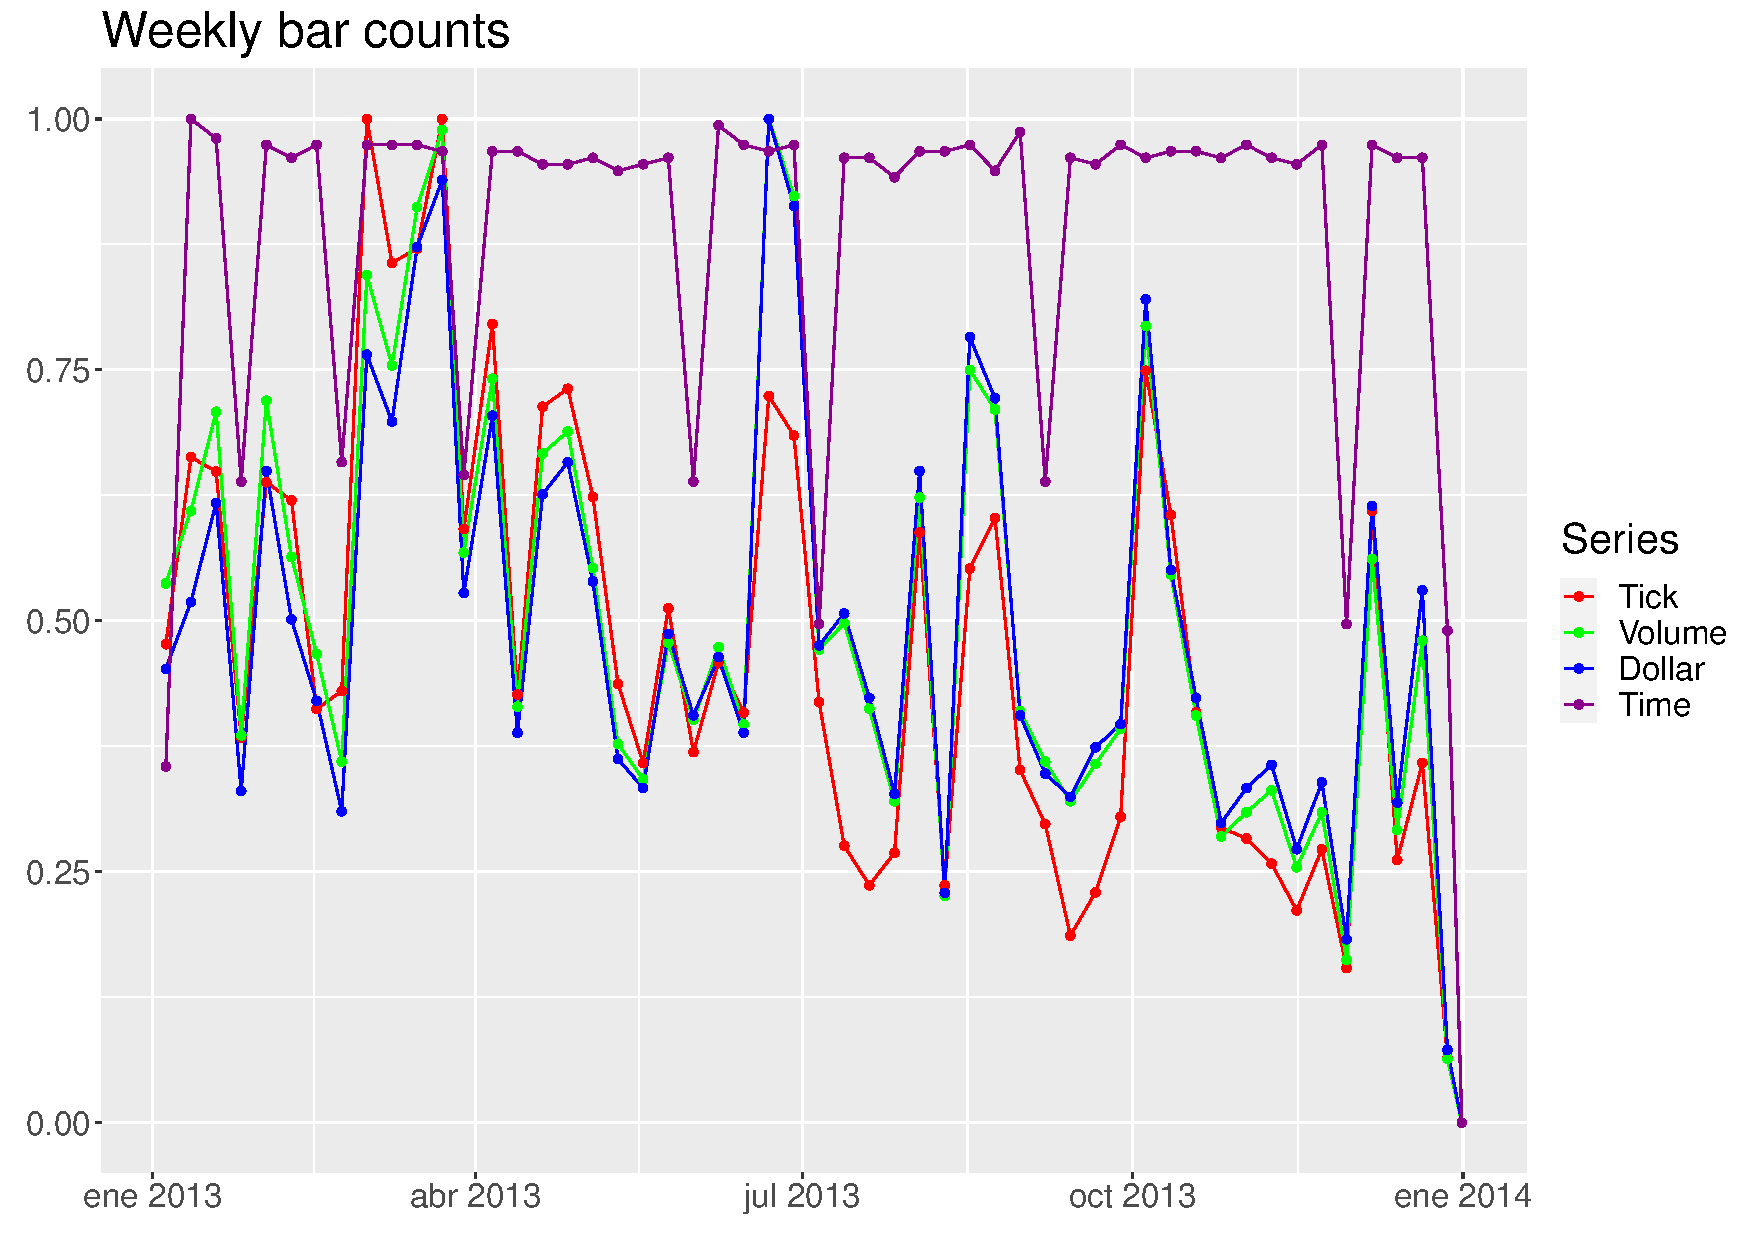
\includegraphics[scale=.35]{img/dataBars/weeklyBarCounts}
	\caption{Normalized weekly bar counts}
	\label{fig:weeklyBarCounts}
\end{figure}

\section{Results}
\label{sec:ARResults}
Having presented the method to create data bars, the obvious question is: 
does sampling the price time series in a different way than time bars give a 
predictive edge?\\

In an attempt to shed some light on the previous question a simple 
autoregressive (AR) model will be used to fit the log-returns obtained via 
tick, volume, dollar and time bars:

\begin{equation*}
	r_k = c + \sum_{i = 1}^{p} \theta_i r_{k - i} + \epsilon_k
\end{equation*}

Note that $r_k$ is no longer indexed via $t$ since it is no longer a time 
series, but a sequence. Additionally, the model order ($p$) will be 
determined with the R package stats \cite{RStats}, which uses the Akaike 
Information Criterion (AIC). This criterion is used to compare different 
models, in this case, different lags $p$.\\

As the datasets obtained with the bars are different, the training data will 
be the whole dataset except the \textbf{last 150 observations}. This number 
is fixed instead of a percentage because datasets have different sizes.\\

The forecasts will be given in a sequential manner. That is, if $N$ is the 
number of bars in the dataset, the model will be trained on the first 
$N - 150$ bars and give a 1-bar forecast ($\widehat{r}_k$). Then, it will be 
trained on the first $N - 150 + 1$ and then give a 1-bar forecast and so on.
\\

Lastly, considering that the datasets are different, an objective way to 
compare the errors $e_k = \widehat{r}_k - r_k$ is the Mean Absolute 
Percentage Error (MAPE):

\begin{equation*}
	\text{MAPE} = \frac{1}{150} \cdot \sum_{k = N - 150 + 1}^N 
	\left| \frac{e_k}{r_k} \right|
\end{equation*}

Note that the metrics used in previous chapters (RMSE, MAD) are 
inappropriate because they are not comparable over different datasets.
\begin{table}[htbp]
\caption{AR results}
\label{tab:ARDataBars}
\centering
\begin{tabular}{ |C{3cm}|C{2cm}|C{2cm}|C{2cm}|C{2cm}| }
	\hline
	 				& Tick & Volume & Dollar & Time\\
	\hline
	Lag ($p$) & 0 & 1 & 10 & 2\\
	MAPE & 1.187730 & 1.129902 & 1.134345 & 2.041313\\
	Improvement & 41.82\% & 44.64\% & 44.43\% & 0\% \\
	\hline
\end{tabular}
\end{table}

As for the results, refer to table \ref{tab:ARDataBars}, which shows the 
chosen lag, the model's MAPE and the improvement on MAPE over the time bar 
model (\textbf{benchmark}). The most striking points are:

\begin{itemize}
	\item The performance of the time model is the worst, with a MAPE of 
	2.04

	\item The tick model, even though the lag used is 0 which means that it 
	predicts a constant, achieves a better MAPE than the time model.
	
	\item The volume and dollar models achieve similar results 
	($\approx 44\%$ improvement) but the complexity of the dollar model is 
	much higher ($p = 10$). Thus, the volume model is preferred.
\end{itemize} 

\section{Conclusions}
This chapter has introduced a useful technique to sample financial data. 
Although it was not possible to recover normality of log-returns through 
this new sampling method, the autoregressive models considered in section 
\ref{sec:ARResults} delivered promising results. The next step would be to 
develop ML Models, that together with other features, would help predict the 
direction of the stock in a determined bar horizon.\\

Additionally, it also remains as future work to design a strategy that is 
able to incorporate data bars. High frequency trading is extremely difficult 
to replicate in an artificial environment since one has to account for 
information lag, order execution, etc. Apart from that, trading with volume 
bars is challenging since it introduces a ``stochastic clock''. That is, if 
one wants to  open a position and the algorithm determines that it should 
be closed after $m$ bars, ones does not know when that event is going to 
happen.